%
%===================================================================================================
%
\documentclass[aspectratio=169]{beamer}
%
%===================================================================================================
%
% Theme and color scheme

\usetheme{Madrid}
\usecolortheme{default}

\definecolor{navy}{RGB}{30,39,97}
\definecolor{darknavy}{RGB}{20,28,61}
\definecolor{darkblue}{RGB}{0,51,102}
\definecolor{accentblue}{RGB}{51,102,170}
\definecolor{lightgray}{RGB}{240,240,245}
\definecolor{darkgreen}{RGB}{0,100,50}
\definecolor{dgreen}{RGB}{45,139,111}
\definecolor{dgray}{RGB}{74,85,104}
\definecolor{lgray}{RGB}{139,149,165}
\definecolor{iceblue}{RGB}{202,220,252}
\definecolor{accent}{RGB}{232,87,74}
\definecolor{darkblue}{RGB}{0,51,102}
\definecolor{darkred}{RGB}{153,0,0}
\definecolor{darkgreen}{RGB}{0,102,51}
\definecolor{lightblue}{RGB}{220,235,245}
\definecolor{lightyellow}{RGB}{255,250,220}
\definecolor{lightgreen}{RGB}{220,245,220}

\setbeamercolor{structure}{fg=darkblue}
\setbeamercolor{frametitle}{bg=darkblue, fg=white}
\setbeamercolor{title}{bg=darkblue, fg=white}
\setbeamercolor{block title}{bg=accentblue, fg=white}
\setbeamercolor{block body}{bg=lightgray}
\setbeamercolor{block title alerted}{bg=red!70!black, fg=white}
\setbeamercolor{block body alerted}{bg=red!5}
\setbeamercolor{block title example}{bg=darkgreen, fg=white}
\setbeamercolor{block body example}{bg=green!5}
%
%===================================================================================================
%
% Packages

\usepackage{amsmath, amssymb, amsfonts, bm, mathtools}
\usepackage{graphicx}
\usepackage{tikz}
\usetikzlibrary{arrows.meta, positioning, calc, decorations.pathreplacing, fit, shapes, matrix}
\usepackage{booktabs}
\usepackage{hyperref}
\usepackage{multicol}

%
%===================================================================================================
%
% Math shortcuts

\newcommand{\E}{\mathbb{E}}
\newcommand{\Var}{\text{Var}}
\newcommand{\Cov}{\text{Cov}}
\newcommand{\R}{\mathbb{R}}

\newcommand{\bz}{\bm{z}}
\newcommand{\bbeta}{\bm{\beta}}
\newcommand{\bff}{\bm{f}}
\newcommand{\br}{\bm{r}}

\newcommand{\Rbar}{\bar{R}}
\newcommand{\Phat}{\hat{P}}
\newcommand{\Lhat}{\hat{\Lambda}}
\newcommand{\Qhat}{\hat{Q}}
\newcommand{\Wone}{W^{(1)}}
\newcommand{\Wzero}{W^{(0)}}
\newcommand{\Pw}{P_{W^{(1)}}}
\newcommand{\norm}[1]{\left\|#1\right\|_F}

\DeclareMathOperator{\tr}{tr}
\DeclareMathOperator{\diag}{diag}
\DeclareMathOperator{\rank}{rank}

%
%===================================================================================================
%
% Navigation

\setbeamertemplate{navigation symbols}{}
\setbeamertemplate{footline}{%
  \hfill\usebeamercolor[fg]{structure}%
  \textbf{Chapter 2} ~--~ \insertframenumber/\inserttotalframenumber%
  \hspace*{6pt}\vspace{3pt}%
}

%
%===================================================================================================
%
% Title page information

\author{Giovanni Della Lunga\\{\footnotesize giovanni.dellalunga@unibo.it}}
\title{Chapter 2\\Factor Models and Dimensionality Reduction}
\subtitle{} % (optional)
\setbeamercovered{transparent} 
\institute{Advanced Topics in Artificial Intelligence} 
\date{Bologna - March, 2026} 
%
%===================================================================================================
%
\begin{document}
%
%===================================================================================================
%
\begin{frame}
\titlepage
\end{frame}
%
%===================================================================================================
%
\AtBeginSection[]
{
  %\begin{frame}<beamer>
  %\footnotesize	
  %\frametitle{Outline}
  %\begin{multicols}{2}
  %\tableofcontents[currentsection]
  %\end{multicols}	  
  %\normalsize
  %\end{frame}
  \begin{frame}
  \vfill
  \centering
  \begin{beamercolorbox}[sep=8pt,center,shadow=true,rounded=true]{title}  	\usebeamerfont{title}\insertsectionhead\par%
  \end{beamercolorbox}
  \vfill
  \end{frame}
}
\AtBeginSubsection{\frame{\subsectionpage}}
%
%===================================================================================================
%
\begin{frame}{Contents}
\begin{multicols}{2}
\tableofcontents[
    sectionstyle=show,
    subsectionstyle=show
]
\end{multicols}
\end{frame}%__________________________________________________________________________
%
\section{Part 1\\Linear Factor Models and PCA}
%__________________________________________________________________________
%
\begin{frame}{Part 1 -- Roadmap}
\begin{enumerate}
    \item The Arbitrage Pricing Theory (Ross, 1976)
    \item The static linear factor model: setup and interpretation
    \item Observable factors: Fama--French models
    \item Latent factors: PCA via Singular Value Decomposition
    \item Consistency of PCA estimators (Bai \& Ng, 2002)
    \item Choosing the number of factors $K$
    \item Observable vs.\ latent, static vs.\ conditional: a taxonomy
    \item Limitations of static models -- motivating what comes next
\end{enumerate}

\vspace{0.5em}
%\textbf{Key reference:} Paper Section 2.1 (equations 5--6) and Section 3.2.
\end{frame}
%__________________________________________________________________________
%
\subsection{APT and the factor model}
%__________________________________________________________________________
%
\begin{frame}{Starting Point: Why Factor Models?}

\textbf{Fundamental question in asset pricing:}\\
Why do different assets earn different average returns?

\vspace{0.7em}
\textbf{Two possible answers:}
\begin{enumerate}
    \item \textbf{Risk compensation:} Higher average returns reflect exposure to systematic risks that investors want to be compensated for bearing.
    \item \textbf{Anomalies / Mispricing:} Some assets are ``cheap'' for reasons unrelated to risk (behavioral biases, institutional frictions, \ldots).
\end{enumerate}

\vspace{0.7em}
Factor models formalize the \textbf{risk compensation} view: all differences in expected returns arise from differences in exposure to a small number of common risk factors.

\vspace{0.5em}
\begin{alertblock}{Central tension in Asset Pricing}
Do asset characteristics predict returns because they proxy for risk exposures (factor structure) or because they capture mispricing (anomalies)?
\end{alertblock}
\end{frame}
%
%..................................................................
%
\begin{frame}{The Arbitrage Pricing Theory (Ross, 1976)}

\textbf{APT assumption:} Asset returns are generated by a \emph{linear factor structure}.

\vspace{0.5em}
If there are $K$ systematic factors, then for asset $i$ at time $t$:
\[
r_{i,t} = \alpha_i + \beta_{i,1}\, f_{1,t} + \beta_{i,2}\, f_{2,t} + \cdots + \beta_{i,K}\, f_{K,t} + u_{i,t}
\]

\textbf{Key ingredients:}
\begin{itemize}
    \item $r_{i,t}$: excess return of asset $i$ (over the risk-free rate)
    \item $f_{k,t}$: return on factor $k$ at time $t$ (systematic shock)
    \item $\beta_{i,k}$: \textbf{loading} of asset $i$ on factor $k$ (risk exposure)
    \item $u_{i,t}$: idiosyncratic return, uncorrelated with factors
    \item $\alpha_i$: intercept (``alpha'' -- pricing error)
\end{itemize}

\vspace{0.5em}
\textbf{APT conclusion:} If no-arbitrage holds and $N$ is large, then $\alpha_i \approx 0$ for all $i$. All expected returns are explained by factor exposures.
\end{frame}
%
%..................................................................
%
\begin{frame}{The Static Linear Factor Model -- Vector Notation}

Stacking across all $N$ assets at time $t$:

$$
\boxed{r_t = \beta\, f_t + u_t}
$$

\vspace{0.3em}
\textbf{Dimensions:}
\begin{center}
\renewcommand{\arraystretch}{1.3}
\begin{tabular}{lcl}
$r_t$ & $\in \R^{N \times 1}$ & vector of excess returns of $N$ assets \\
$f_t$ & $\in \R^{K \times 1}$ & vector of $K$ factor returns \\
$\beta$ & $\in \R^{N \times K}$ & matrix of factor loadings \\
$u_t$ & $\in \R^{N \times 1}$ & idiosyncratic errors \\
\end{tabular}
\end{center}

\vspace{0.5em}
\textbf{Assumptions:}
\begin{itemize}
    \item $\E[u_t | f_t] = 0$ \quad (idiosyncratic risk is orthogonal to factors)
    \item $\Cov(u_{i,t}, u_{j,t}) \approx 0$ for $i \neq j$ \quad (approximate factor structure)
    \item $\beta$ is \textbf{constant over time} \quad (static loadings)
\end{itemize}
\end{frame}
%
%..................................................................
%
\begin{frame}{Interpretation of Each Component}

\textbf{Factors} $f_t$:
\begin{itemize}
    \item Sources of \emph{systematic} (non-diversifiable) risk
    \item Examples: market return, recession shocks, interest rate changes
    \item Can be \textbf{observable} (traded portfolios) or \textbf{latent} (unknown)
\end{itemize}

\vspace{0.5em}
\textbf{Loadings} $\beta_i$:
\begin{itemize}
    \item How much asset $i$ ``co-moves'' with each factor
    \item $\beta_{i,k}$ high $\Rightarrow$ asset $i$ is very sensitive to factor $k$
    \item Determines risk \emph{and} expected return
\end{itemize}

\vspace{0.5em}
\textbf{Idiosyncratic error} $u_{i,t}$:
\begin{itemize}
    \item Firm-specific shock (CEO scandal, product recall, \ldots)
    \item \textbf{Diversifiable:} in a portfolio of many stocks, $\frac{1}{N}\sum_i u_{i,t} \to 0$
\end{itemize}

\end{frame}
%
%..................................................................
%
\begin{frame}{The Pricing Implication: Security Market Line}

Under no-arbitrage (APT), all expected excess returns are compensation for factor risk:

\begin{block}{Asset Pricing Restriction}
\vspace{-0.5em}
\[
\E[r_{i,t}] = \beta_i' \lambda
\]
where $\lambda = \E[f_t]$ is the $K \times 1$ vector of \textbf{factor risk premia}.
\end{block}

\vspace{0.3em}
\textbf{What this says:}
\begin{itemize}
    \item An asset's expected return depends \textbf{only} on its factor exposures $\beta_i$
    \item Each unit of exposure to factor $k$ is compensated at rate $\lambda_k$
    \item There is \textbf{no alpha}: $\alpha_i = \E[r_{i,t}] - \beta_i'\lambda = 0$
\end{itemize}

\vspace{0.5em}
\textbf{If $\alpha_i \neq 0$} for some asset $i$, either:
\begin{enumerate}
    \item The model is misspecified (wrong factors or wrong $\beta$), or
    \item There is genuine mispricing (anomaly)
\end{enumerate}
\end{frame}
%
%..................................................................
%
\begin{frame}{Graphical Intuition: One Factor (CAPM)}

\begin{center}
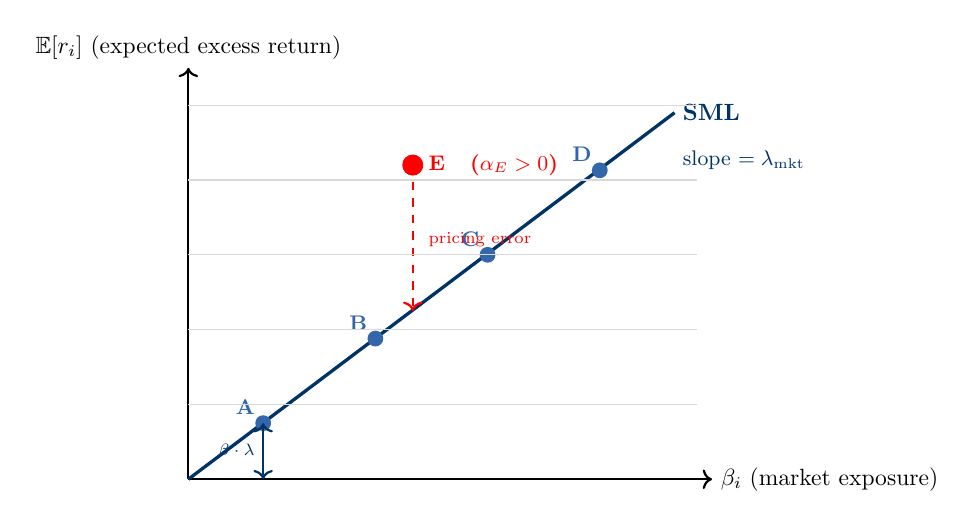
\begin{tikzpicture}[scale=0.95, every node/.style={scale=0.85}]
  \draw[->, thick] (0,0) -- (7,0) node[right] {$\beta_i$ (market exposure)};
  \draw[->, thick] (0,0) -- (0,5.5) node[above] {$\E[r_i]$ (expected excess return)};
  
  % SML line
  \draw[very thick, darkblue] (0,0) -- (6.5,4.9);
  \node[darkblue, right, font=\bfseries] at (6.5,4.9) {SML};
  \node[darkblue, below right, font=\small] at (6.5, 4.5) {slope $= \lambda_{\text{mkt}}$};
  
  % Points on the line
  \foreach \x/\y/\lab in {1.0/0.75/A, 2.5/1.88/B, 4.0/3.00/C, 5.5/4.13/D}{
    \fill[accentblue] (\x,\y) circle (3pt);
    \node[accentblue, above left, font=\small\bfseries] at (\x,\y) {\lab};
  }
  
  % Mispriced asset
  \fill[red] (3.0,4.2) circle (4pt);
  \node[red, right, font=\small\bfseries] at (3.1,4.2) {E ~~($\alpha_E > 0$)};
  \draw[dashed, red, thick, ->] (3.0,4.2) -- (3.0,2.25);
  \node[red, right, font=\scriptsize] at (3.1, 3.2) {pricing error};
  
  % Lambda label
  \draw[<->, darkblue, thick] (1.0, 0) -- (1.0, 0.75);
  \node[darkblue, left, font=\scriptsize] at (1.0, 0.375) {$\beta \cdot \lambda$};
  
  % Grid
  \foreach \y in {1,2,3,4,5}{
    \draw[gray!30, thin] (0,\y) -- (6.8,\y);
  }
\end{tikzpicture}
\end{center}

\vspace{0.3em}
Assets on the Security Market Line: $\alpha = 0$ (correctly priced).\\
Asset E is above the line: it earns more than justified by its $\beta$ $\Rightarrow$ $\alpha_E > 0$.
\end{frame}
%
%..................................................................
%
\begin{frame}{Multi-Factor Generalization}

With $K > 1$ factors, the SML becomes a \emph{hyperplane} in $(K+1)$-dimensional space:
\[
\E[r_i] = \beta_{i,1}\lambda_1 + \beta_{i,2}\lambda_2 + \cdots + \beta_{i,K}\lambda_K
\]

\vspace{0.5em}
\textbf{Example with $K = 3$:}
\[
\E[r_i] = \underbrace{\beta_{i,\text{mkt}}}_{\text{market exposure}} \cdot \underbrace{\lambda_{\text{mkt}}}_{\approx 6\%/\text{yr}} + \underbrace{\beta_{i,\text{smb}}}_{\text{size exposure}} \cdot \underbrace{\lambda_{\text{smb}}}_{\approx 2\%/\text{yr}} + \underbrace{\beta_{i,\text{hml}}}_{\text{value exposure}} \cdot \underbrace{\lambda_{\text{hml}}}_{\approx 3\%/\text{yr}}
\]

\vspace{0.5em}
\textbf{Key question:} What are the ``right'' factors?

\vspace{0.3em}
\begin{columns}[T]
\column{0.48\textwidth}
\begin{block}{Approach 1: Observable factors}
Specify factors from economic theory or empirical regularities (Fama--French).
\end{block}

\column{0.48\textwidth}
\begin{block}{Approach 2: Latent factors}
Extract factors statistically from the data (PCA).
\end{block}
\end{columns}
\end{frame}
%__________________________________________________________________________
%
\subsection{Observable factor models (Fama-French)}
%__________________________________________________________________________
%
\begin{frame}{Observable Factor Models: The Fama--French Tradition}

\textbf{Idea:} Construct factors as returns on \emph{long-short portfolios} sorted by firm characteristics.

\vspace{0.7em}
\begin{center}
\renewcommand{\arraystretch}{1.4}
\begin{tabular}{llp{7cm}}
\toprule
\textbf{Factor} & \textbf{Acronym} & \textbf{Construction} \\
\midrule
Market & MKT & Value-weighted market return minus risk-free rate \\
Size & SMB & Small minus Big: return on small-cap portfolio minus large-cap portfolio \\
Value & HML & High minus Low: return on high book-to-market portfolio minus low B/M portfolio \\
\bottomrule
\end{tabular}
\end{center}

\vspace{0.5em}
These three factors define the \textbf{Fama--French three-factor model} (FF3, 1993).
\end{frame}
%
%..................................................................
%
\begin{frame}{Extending FF3: Five and Six Factor Models}
\small
\begin{center}
\renewcommand{\arraystretch}{1.35}
\begin{tabular}{llp{6.5cm}}
\toprule
\textbf{Model} & \textbf{Factors} & \textbf{What's added} \\
\midrule
CAPM & MKT & Single factor \\
FF3 & MKT, SMB, HML & Size + Value \\
Carhart 4F & MKT, SMB, HML, UMD & + Momentum (Up Minus Down) \\
FF5 & MKT, SMB, HML, RMW, CMA & + Profitability (Robust Minus Weak), + Investment (Conservative Minus Aggressive) \\
FF6 & MKT, SMB, HML, RMW, CMA, UMD & + Momentum \\
\bottomrule
\end{tabular}
\end{center}

\vspace{0.7em}
%\textbf{In the paper:} FF models with $K = 1$ to $6$ factors %are used as benchmarks (Section 3.2). Factor returns from Ken %French's website.
\end{frame}
%
%..................................................................
%
\begin{frame}{How Are FF Betas Estimated?}

Given observable factors $f_t = (f_{1,t}, \ldots, f_{K,t})'$, for each asset $i$ run a \textbf{time-series regression}:
\[
r_{i,t} = \alpha_i + \beta_{i,1} f_{1,t} + \cdots + \beta_{i,K} f_{K,t} + u_{i,t}, \qquad t = 1, \ldots, T
\]

\vspace{0.3em}
\textbf{Estimation:} OLS gives $\hat{\beta}_i = (\hat{\beta}_{i,1}, \ldots, \hat{\beta}_{i,K})'$ for each stock $i$.

\vspace{0.7em}
\textbf{Practical issues:}
\begin{itemize}
    \item Need enough time-series data per stock (typically 60 months rolling window)
    \item $\hat{\beta}_i$ is \textbf{constant} within each estimation window
    \item Must re-estimate periodically $\Rightarrow$ crude step-function approximation to time variation
    \item Poor for short-lived stocks (IPOs, delistings) -- unbalanced panel problem
\end{itemize}

\vspace{0.5em}
%\begin{alertblock}{Key limitation in the paper's empirical design}
%The paper re-estimates parameters only \textbf{once per year}. With static betas, this infrequent updating severely hurts FF models (Table 1: FF6 total $R^2 = -6.1\%$ on individual stocks!).
%\end{alertblock}
\end{frame}
%
%..................................................................
%
\begin{frame}{Strengths and Weaknesses of Observable Factor Models}

\begin{columns}[T]
\column{0.48\textwidth}
\begin{exampleblock}{Strengths}
\begin{itemize}
    \item Economically interpretable factors
    \item Simple estimation (OLS)
    \item Long history of empirical validation
    \item Factors are tradeable portfolios $\Rightarrow$ direct economic meaning
    \item Widely used in industry and academia
\end{itemize}
\end{exampleblock}

\column{0.48\textwidth}
\begin{alertblock}{Weaknesses}
\begin{itemize}
    \item \textbf{Which factors?} The ``factor zoo'' problem -- hundreds of proposed factors
    \item \textbf{Static betas:} Cannot capture time-variation in risk exposures
    \item \textbf{No conditioning information:} Ignores firm characteristics
    \item \textbf{Ad hoc factor selection:} No guarantee these are the ``right'' factors
    %\item \textbf{Poor cross-sectional fit} for large panels (Table 1)
\end{itemize}
\end{alertblock}
\end{columns}
\end{frame}
%__________________________________________________________________________
%
\subsection{Latent factors and PCA}
%__________________________________________________________________________
%
\begin{frame}{Latent Factors: The PCA Approach}

\textbf{Alternative:} Don't pre-specify factors. Let the \emph{data} tell us what the common sources of variation are.

\vspace{0.5em}
\textbf{Idea:} Find the $K$ directions in return space that explain the most \emph{common variance} across all $N$ assets.

\vspace{0.7em}
\textbf{Setup:} Stack the factor model over all $T$ periods:
\[
R = \beta\, F + U
\]

\begin{center}
\renewcommand{\arraystretch}{1.2}
\begin{tabular}{lcl}
$R$ & $\in \R^{N \times T}$ & matrix of all excess returns \\
$\beta$ & $\in \R^{N \times K}$ & loadings matrix \\
$F$ & $\in \R^{K \times T}$ & factors matrix \\
$U$ & $\in \R^{N \times T}$ & idiosyncratic errors \\
\end{tabular}
\end{center}

\vspace{0.5em}
\textbf{Problem:} Both $\beta$ and $F$ are unknown. We need to estimate them \emph{simultaneously} from $R$ alone. This is an \textbf{unsupervised} problem.
\end{frame}
%
%..................................................................
%
\begin{frame}{PCA via Singular Value Decomposition (SVD)}

\textbf{Step 1:} Demean the returns: $\bar{R} = R - \bar{r}\,\iota'$ where $\bar{r} = \frac{1}{T}\sum_t r_t$.

\vspace{0.5em}
\textbf{Step 2:} Compute the SVD of $\bar{R}$:

$$
\bar{R} = \hat{P}\,\hat{\Lambda}\,\hat{Q} + \hat{U}
$$

\vspace{0.3em}
where:
\begin{itemize}
    \item $\hat{P} \in \R^{N \times K}$: left singular vectors $=$ \textbf{estimated factor loadings}
    \item $\hat{\Lambda} \in \R^{K \times K}$: diagonal matrix of singular values ($\sigma_1 \geq \sigma_2 \geq \cdots \geq \sigma_K > 0$)
    \item $\hat{Q} \in \R^{K \times T}$: right singular vectors $=$ \textbf{estimated factors}
    \item $\hat{U} \in \R^{N \times T}$: residual matrix
\end{itemize}

%\vspace{0.5em}
%\textbf{Key property:} $\hat{P}\hat{\Lambda}\hat{Q}$ is the \textbf{best rank-$K$ approximation} of $\bar{R}$ in the Frobenius norm (Eckart--Young--Mirsky theorem).
\end{frame}
%
%..................................................................
%
\begin{frame}{SVD: Visual Representation}

\begin{center}
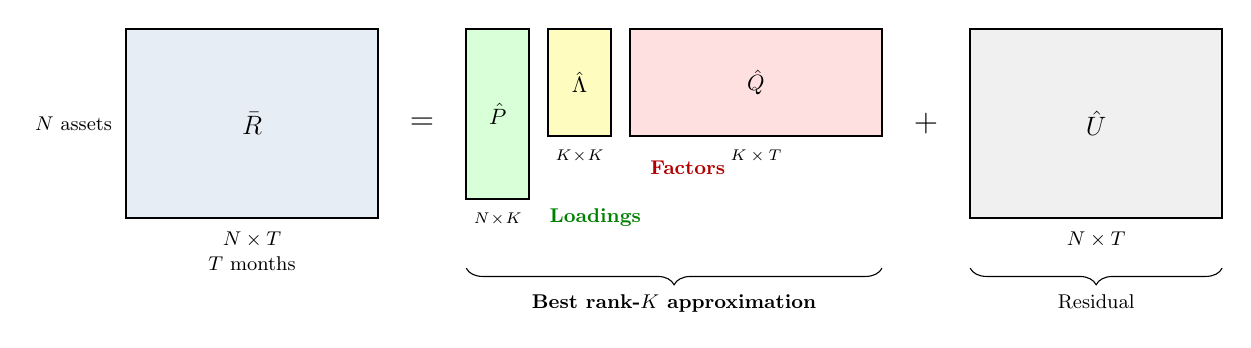
\begin{tikzpicture}[scale=0.8, every node/.style={scale=0.8}]
  % R matrix
  \draw[fill=accentblue!12, thick] (0,0) rectangle (4.0,3.0);
  \node[font=\large] at (2.0, 1.5) {$\bar{R}$};
  \node[below, font=\small] at (2.0,-0.1) {$N \times T$};
  \node[left, font=\small] at (-0.1,1.5) {$N$ assets};
  \node[below, font=\small] at (2.0,-0.5) {$T$ months};
  
  \node[font=\Large] at (4.7, 1.5) {$=$};
  
  % P matrix
  \draw[fill=green!15, thick] (5.4,0.3) rectangle (6.4,3.0);
  \node at (5.9, 1.65) {$\hat{P}$};
  \node[below, font=\scriptsize] at (5.9,0.2) {$N\!\times\!K$};
  
  % Lambda matrix
  \draw[fill=yellow!25, thick] (6.7,1.3) rectangle (7.7,3.0);
  \node at (7.2, 2.15) {$\hat{\Lambda}$};
  \node[below, font=\scriptsize] at (7.2,1.2) {$K\!\times\!K$};
  
  % Q matrix
  \draw[fill=red!12, thick] (8.0,1.3) rectangle (12.0,3.0);
  \node at (10.0, 2.15) {$\hat{Q}$};
  \node[below, font=\scriptsize] at (10.0,1.2) {$K \times T$};
  
  \node[font=\Large] at (12.7, 1.5) {$+$};
  
  % U matrix
  \draw[fill=gray!12, thick] (13.4,0) rectangle (17.4,3.0);
  \node[font=\large] at (15.4, 1.5) {$\hat{U}$};
  \node[below, font=\small] at (15.4,-0.1) {$N \times T$};
  
  % Braces
  \draw[decorate, decoration={brace, amplitude=6pt, mirror}] (5.4,-0.8) -- (12.0,-0.8);
  \node[below, font=\small\bfseries] at (8.7,-1.1) {Best rank-$K$ approximation};
  
  \draw[decorate, decoration={brace, amplitude=6pt, mirror}] (13.4,-0.8) -- (17.4,-0.8);
  \node[below, font=\small] at (15.4,-1.1) {Residual};
  
  % Annotations
  \node[green!50!black, font=\small\bfseries, right] at (6.6, 0.0) {Loadings};
  \node[red!70!black, font=\small\bfseries, right] at (8.2, 0.8) {Factors};
\end{tikzpicture}
\end{center}

\vspace{0.5em}
PCA selects the $K$ directions that capture the \textbf{maximum} amount of common variation in the return panel.
\end{frame}
%
%..................................................................
%
\begin{frame}{Equivalent Formulation via Covariance Matrix}
\small
\textbf{Alternative (equivalent) approach:}

\vspace{0.3em}
\textbf{Step 1:} Estimate the covariance matrix of returns:
\[
\hat{\Sigma} = \frac{1}{T}\bar{R}\,\bar{R}'  \qquad (N \times N)
\]

\textbf{Step 2:} Eigenvalue decomposition:
\[
\hat{\Sigma} = \hat{P}\,\hat{D}\,\hat{P}' + \text{residual}
\]
where $\hat{D} = \hat{\Lambda}^2 / T$ contains the eigenvalues.

\vspace{0.7em}
\textbf{Connection:}
\begin{itemize}
    \item Eigenvectors of $\hat{\Sigma}$ $=$ left singular vectors of $\bar{R}$ $=$ PCA loadings $\hat{P}$
    \item Eigenvalues of $\hat{\Sigma}$ $=$ squared singular values / $T$ $=$ variance explained by each PC
\end{itemize}

\vspace{0.5em}
\begin{exampleblock}{No-arbitrage variant}
To impose the zero-intercept restriction (no alpha), apply PCA to the \emph{uncentered second moment matrix} $\frac{1}{T}R\,R'$ instead of the (centered) covariance.
\end{exampleblock}
\end{frame}
%
%..................................................................
%
\begin{frame}{What PCA ``Sees'' in the Data}

\textbf{Intuition:} Each principal component captures one independent dimension of co-movement.

\vspace{0.7em}
\begin{columns}[T]
\column{0.48\textwidth}
\textbf{PC 1:} Typically the ``market factor''
\begin{itemize}
    \item Most stocks move together with the overall market
    \item Explains the largest fraction of variance (typically 20--30\% for individual stocks)
\end{itemize}

\vspace{0.3em}
\textbf{PC 2:} Often captures size or industry effects
\begin{itemize}
    \item Orthogonal to PC1 by construction
    \item Smaller contribution to total variance
\end{itemize}

\column{0.48\textwidth}
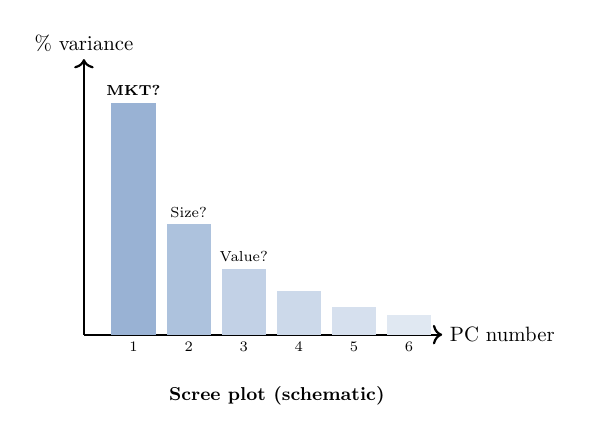
\begin{tikzpicture}[scale=0.7, every node/.style={scale=0.75}]
  \draw[->, thick] (0,0) -- (6.5,0) node[right] {PC number};
  \draw[->, thick] (0,0) -- (0,5) node[above] {\% variance};
  
  % Scree plot
  \fill[accentblue!50] (0.5,0) rectangle (1.3, 4.2);
  \fill[accentblue!40] (1.5,0) rectangle (2.3, 2.0);
  \fill[accentblue!30] (2.5,0) rectangle (3.3, 1.2);
  \fill[accentblue!25] (3.5,0) rectangle (4.3, 0.8);
  \fill[accentblue!20] (4.5,0) rectangle (5.3, 0.5);
  \fill[accentblue!15] (5.5,0) rectangle (6.3, 0.35);
  
  \node[below, font=\scriptsize] at (0.9,0) {1};
  \node[below, font=\scriptsize] at (1.9,0) {2};
  \node[below, font=\scriptsize] at (2.9,0) {3};
  \node[below, font=\scriptsize] at (3.9,0) {4};
  \node[below, font=\scriptsize] at (4.9,0) {5};
  \node[below, font=\scriptsize] at (5.9,0) {6};
  
  \node[above, font=\scriptsize\bfseries] at (0.9,4.2) {MKT?};
  \node[above, font=\scriptsize] at (1.9,2.0) {Size?};
  \node[above, font=\scriptsize] at (2.9,1.2) {Value?};
  
  \node[below, font=\small\bfseries] at (3.5, -0.8) {Scree plot (schematic)};
\end{tikzpicture}
\end{columns}

\vspace{0.5em}
\textbf{Important:} PCA factors are \emph{statistical} objects -- they need not correspond to named economic factors. Interpretation requires additional analysis.
\end{frame}
%
%..................................................................
%
\begin{frame}{A Numerical Intuition: 2D Example}

\begin{center}
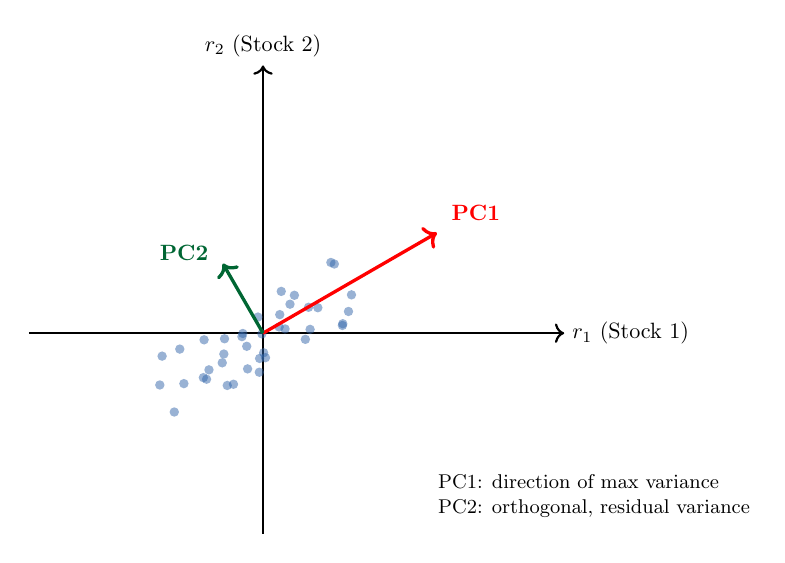
\begin{tikzpicture}[scale=0.85, every node/.style={scale=0.8}]
  % Axes
  \draw[->, thick] (-3.5,0) -- (4.5,0) node[right] {$r_1$ (Stock 1)};
  \draw[->, thick] (0,-3) -- (0,4) node[above] {$r_2$ (Stock 2)};
  
  % Random data cloud (elongated ellipse)
  \foreach \i in {1,...,40}{
    \pgfmathsetmacro{\a}{rand*1.8}
    \pgfmathsetmacro{\b}{rand*0.5}
    \pgfmathsetmacro{\x}{\a*cos(30) - \b*sin(30)}
    \pgfmathsetmacro{\y}{\a*sin(30) + \b*cos(30)}
    \fill[accentblue, opacity=0.5] (\x,\y) circle (2pt);
  }
  
  % PC1 direction
  \draw[very thick, red, ->] (0,0) -- (3.0*0.866, 3.0*0.5);
  \node[red, font=\bfseries, right] at (2.7, 1.8) {PC1};
  
  % PC2 direction
  \draw[very thick, darkgreen, ->] (0,0) -- (-1.2*0.5, 1.2*0.866);
  \node[darkgreen, font=\bfseries, left] at (-0.7, 1.2) {PC2};
  
  % Annotation
  \node[below right, font=\small, align=left] at (2.5, -2.0) {
    PC1: direction of max variance\\
    PC2: orthogonal, residual variance
  };
\end{tikzpicture}
\end{center}
\footnotesize
With $N = 2$ stocks and $K = 1$ factor: the first PC captures the main direction of co-movement. The second PC captures residual, orthogonal variation.
\end{frame}
%
%..................................................................
%
\begin{frame}{Rotation Indeterminacy -- Why It Matters}

\textbf{Fact:} If $(\beta, F)$ is a valid factorization, then so is $(\beta H, H^{-1} F)$ for any invertible $H$:
\[
r_t = \beta\, f_t + u_t = (\beta H)(H^{-1}f_t) + u_t
\]
The product $\beta f_t$ is unchanged!

\vspace{0.7em}
\textbf{Consequences:}
\begin{itemize}
    \item PCA factors are \textbf{not uniquely identified} -- they span the same space as the ``true'' factors, but may be arbitrary rotations
    \item We can identify the factor \emph{space} (column space of $\beta$) but not individual factors
    \item Interpretation requires additional restrictions or rotation criteria
\end{itemize}

%\vspace{0.5em}
%\textbf{In the paper:} The identifying restrictions used are:
%\[
%\Gamma\Gamma' = I_K, \qquad FF' \text{ diagonal with descending entries}, \qquad F\iota \geq 0
%\]
%These pin down a unique rotation without imposing economic restrictions.
\end{frame}
%__________________________________________________________________________
%
\subsection{Choosing K}
%__________________________________________________________________________
%
\begin{frame}{Choosing the Number of Factors $K$}

\textbf{How many factors do we need?}

\vspace{0.5em}
\textbf{Several approaches in the literature:}
\begin{enumerate}
    \item \textbf{Information criteria} (Bai \& Ng, 2002):
    \[
    IC(K) = \ln\left(\frac{1}{NT}\sum_{i,t}\hat{u}_{i,t}^2\right) + K \cdot g(N,T)
    \]
    where $g(N,T)$ is a penalty that grows with $K$ (analogous to AIC/BIC).
    
    \vspace{0.3em}
    \item \textbf{Eigenvalue ratio test} (Ahn \& Horenstein, 2013):
    \[
    ER(K) = \frac{\hat{\lambda}_K}{\hat{\lambda}_{K+1}} \qquad \text{(maximize over } K\text{)}
    \]
    Large ratio $\Rightarrow$ big gap between factor $K$ and factor $K+1$.
    
    \vspace{0.3em}
    \item \textbf{Cross-validation} (used in the paper):
    Treat $K$ as a \textbf{tuning parameter} and select via out-of-sample validation performance.
\end{enumerate}
\end{frame}
%
%..................................................................
%
\begin{frame}{Cross-Validation for $K$: The ML Approach}

\begin{center}
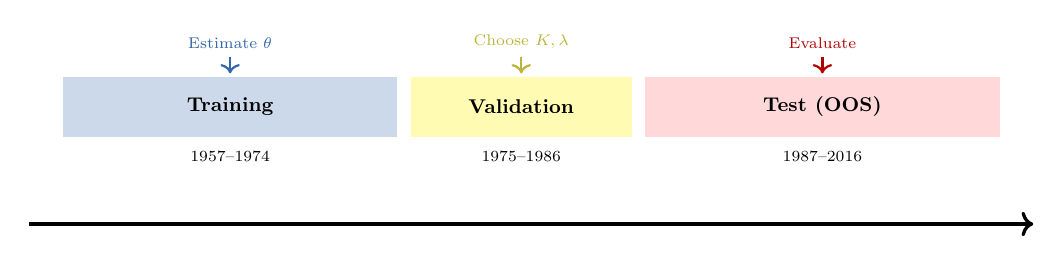
\begin{tikzpicture}[scale=0.85, every node/.style={scale=0.8}]
  % Timeline
  \draw[very thick, ->] (0,-1) -- (15,-1);
  
  % Training
  \fill[accentblue!25] (0.5,0.3) rectangle (5.5,1.2);
  \node[font=\small\bfseries] at (3.0, 0.75) {Training};
  \node[font=\scriptsize, below] at (3.0, 0.2) {1957--1974};
  
  % Validation
  \fill[yellow!30] (5.7,0.3) rectangle (9.0,1.2);
  \node[font=\small\bfseries] at (7.35, 0.75) {Validation};
  \node[font=\scriptsize, below] at (7.35, 0.2) {1975--1986};
  
  % Test
  \fill[red!15] (9.2,0.3) rectangle (14.5,1.2);
  \node[font=\small\bfseries] at (11.85, 0.75) {Test (OOS)};
  \node[font=\scriptsize, below] at (11.85, 0.2) {1987--2016};
  
  % Arrows
  \draw[->, thick, accentblue] (3.0, 1.5) -- (3.0, 1.25);
  \node[above, font=\scriptsize, accentblue] at (3.0, 1.5) {Estimate $\theta$};
  
  \draw[->, thick, yellow!70!black] (7.35, 1.5) -- (7.35, 1.25);
  \node[above, font=\scriptsize, yellow!70!black] at (7.35, 1.5) {Choose $K, \lambda$};
  
  \draw[->, thick, red!70!black] (11.85, 1.5) -- (11.85, 1.25);
  \node[above, font=\scriptsize, red!70!black] at (11.85, 1.5) {Evaluate};
\end{tikzpicture}
\end{center}

\vspace{0.5em}
\begin{itemize}
    \item Try $K = 1, 2, 3, 4, 5, 6$
    \item For each $K$: estimate the model on training data, evaluate on validation data
    \item Select the $K$ that gives the best validation performance
    \item Report final results on the \textbf{test set only} (never used for estimation or tuning)
\end{itemize}

%\vspace{0.3em}
%\textbf{Paper's finding:} Models generally improve up to $K = 5$ or $6$; deeper architectures benefit more from additional %factors.
\end{frame}
%__________________________________________________________________________
%
\subsection{Limitations of Static Models and Main Takeaways}
%__________________________________________________________________________
%
\begin{frame}{Taxonomy of Factor Models (What We Know So Far)}

\begin{center}
\renewcommand{\arraystretch}{1.5}
\begin{tabular}{p{3.0cm} p{4.5cm} p{4.5cm}}
\toprule
 & \textbf{Observable Factors (FF)} & \textbf{Latent Factors (PCA)} \\
\midrule
\textbf{Factors} & Pre-specified traded portfolios (MKT, SMB, HML, \ldots) & Data-driven via SVD \\
\textbf{Betas} & Static (constant) & Static (constant) \\
\textbf{Cond.\ info} & None & None \\
\textbf{Estimation} & OLS time-series regression & Eigenvalue decomposition \\
\textbf{Interpretation} & Clear economic meaning & Statistical (needs rotation) \\
\textbf{Flexibility} & Low & Moderate \\
\textbf{Missing data} & Handled naturally & Requires EM algorithm \\
\bottomrule
\end{tabular}
\end{center}

\vspace{0.3em}
\textbf{Common weakness:} Both assume $\beta$ is constant. Neither uses firm characteristics.
\end{frame}
%
%..................................................................
%
\begin{frame}{Empirical Evidence: How Do Static Models Perform?}

\textbf{Table 1 of the paper:} Out-of-sample total $R^2$ (\%) for individual stocks $r_t$.

\vspace{0.5em}
\begin{center}
\renewcommand{\arraystretch}{1.2}
\begin{tabular}{lcccccc}
\toprule
\textbf{Model} & $K=1$ & $K=2$ & $K=3$ & $K=4$ & $K=5$ & $K=6$ \\
\midrule
FF & 4.8 & 4.6 & 3.4 & 0.1 & $-2.3$ & $-6.1$ \\
PCA & 7.3 & 3.3 & 5.0 & 5.3 & 4.2 & 3.9 \\
\midrule
\textcolor{gray}{IPCA} & \textcolor{gray}{11.2} & \textcolor{gray}{12.4} & \textcolor{gray}{13.3} & \textcolor{gray}{13.7} & \textcolor{gray}{14.3} & \textcolor{gray}{14.5} \\
\textcolor{gray}{CA2} & \textcolor{gray}{10.7} & \textcolor{gray}{11.8} & \textcolor{gray}{12.6} & \textcolor{gray}{13.2} & \textcolor{gray}{13.6} & \textcolor{gray}{13.8} \\
\bottomrule
\end{tabular}
\end{center}

\vspace{0.3em}
\textbf{Observations:}
\begin{itemize}
    \item FF models \emph{deteriorate} as $K$ increases (overfitting with static betas!)
    \item FF6 has \textbf{negative} $R^2$: worse than predicting zero for every stock
    \item PCA is better but plateaus around 5--7\%
    \item Conditional models (grey rows) are dramatically better -- we'll see why in Part 3
\end{itemize}
\end{frame}
%
%..................................................................
%
\begin{frame}{Preview: What We Need}

\textbf{The limitations we've identified:}

\vspace{0.5em}
\begin{enumerate}
    \item \textbf{Static betas} miss time-variation in risk exposures
    
    $\Rightarrow$ \textit{Solution:} Make $\beta$ a function of observable characteristics $z_{i,t-1}$
    
    \vspace{0.3em}
    \item \textbf{Observable factors} may not be the ``right'' factors
    
    $\Rightarrow$ \textit{Solution:} Use latent factors estimated from the data
    
    \vspace{0.3em}
    \item \textbf{Linear models} may not capture the true relationship between characteristics and betas
    
    $\Rightarrow$ \textit{Solution:} Allow nonlinear mappings (neural networks)
    
    \vspace{0.3em}
    \item \textbf{Dimensionality reduction} should incorporate both returns and characteristics
    
    $\Rightarrow$ \textit{Solution:} The \emph{conditional autoencoder} -- combining all of the above
\end{enumerate}

\vspace{0.5em}
\textbf{Roadmap:}
\begin{itemize}
    \item Part 2: PCA $=$ linear autoencoder (the mathematical bridge)
    \item Part 3: Adding conditioning information $\Rightarrow$ IPCA, then going nonlinear
\end{itemize}
\end{frame}
%
%..................................................................
%
\begin{frame}{Part 1 -- Summary}

\begin{enumerate}
    \item The \textbf{APT} (Ross, 1976) posits that returns follow a linear factor structure $r_t = \beta f_t + u_t$, and under no-arbitrage, $\E[r_i] = \beta_i' \lambda$.
    
    \vspace{0.3em}
    \item \textbf{Observable factor models} (Fama--French) use pre-specified traded portfolios. Economically interpretable, but factors are ad hoc and betas are static.
    
    \vspace{0.3em}
    \item \textbf{PCA} extracts latent factors via SVD: $\bar{R} = \hat{P}\hat{\Lambda}\hat{Q} + \hat{U}$. Data-driven, consistent as $N,T \to \infty$ (Bai \& Ng), but still assumes static loadings.
    
    \vspace{0.3em}
    \item The number of factors $K$ can be chosen via information criteria, eigenvalue ratios, or cross-validation (the paper's approach).
    
    \vspace{0.3em}
    \item \textbf{Empirically:} Static models (both FF and PCA) perform poorly on individual stocks with infrequent re-estimation and a large cross-section. This motivates \emph{conditional} and \emph{nonlinear} factor models.
\end{enumerate}

\vspace{0.5em}
\textbf{Next (Part 2):} We'll see that PCA is a special case of autoencoders, opening the door to more powerful architectures.
\end{frame}
%__________________________________________________________________________
%
\section{Part 2\\From PCA to the Linear Autoencoder}
%__________________________________________________________________________
%
\begin{frame}{Part 2 -- Roadmap}
\begin{enumerate}
    \item Quick recap: what is an autoencoder?
    \item The standard autoencoder architecture
    \item The encoder--decoder paradigm and the bottleneck
    \item Writing the linear autoencoder mathematically
    \item linear AE $=$ PCA
    \item loadings, factors, and rotation
    \item What changes when we add nonlinearity?
    \item Deep autoencoders: going beyond PCA
    \item The hierarchy: PCA $\subset$ Linear AE $\subset$ Nonlinear AE $\subset$ Conditional AE
\end{enumerate}
\end{frame}
%__________________________________________________________________________
%
\subsection{Autoencoder architecture}
%__________________________________________________________________________
%
\begin{frame}{What Is an Autoencoder?}

\textbf{From Lecture 1:} An autoencoder is a neural network trained to \emph{reconstruct its own input}.

\vspace{0.5em}
\begin{block}{Definition}
An autoencoder maps input $x$ through a bottleneck and attempts to produce output $\hat{x} \approx x$.
\[
x \xrightarrow{\text{encoder}} h \xrightarrow{\text{decoder}} \hat{x} \approx x
\]
\end{block}

\vspace{0.3em}
\textbf{Why is this useful?}
\begin{itemize}
    \item The bottleneck $h$ (hidden layer with $K \ll N$ neurons) forces a \emph{compressed representation}
    \item If the network can reconstruct $x$ well from $h$, then $h$ captures the essential information
    \item This is an \textbf{unsupervised} method: no labels needed, only the data itself
\end{itemize}

%\vspace{0.5em}
%\textbf{In our context:} $x = r_t$ (returns of $N$ stocks), $h %= f_t$ (K latent factors), $\hat{x} = \hat{r}_t$ (reconstructed returns).
\end{frame}
%
%..................................................................
%
\begin{frame}{Standard Autoencoder Architecture}

\begin{center}
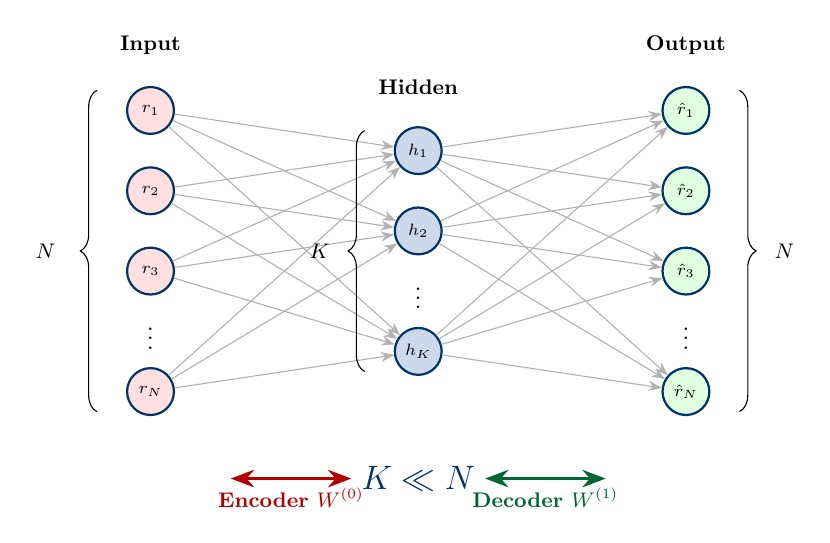
\begin{tikzpicture}[
    neuron/.style={circle, draw=darkblue, thick, minimum size=7mm, inner sep=0, font=\scriptsize},
    >=Stealth, scale=0.85, every node/.style={scale=0.85}
]
  % Input layer
  \node[neuron, fill=red!12] (I1) at (0, 0) {$r_1$};
  \node[neuron, fill=red!12] (I2) at (0, -1.2) {$r_2$};
  \node[neuron, fill=red!12] (I3) at (0, -2.4) {$r_3$};
  \node at (0, -3.3) {$\vdots$};
  \node[neuron, fill=red!12] (IN) at (0, -4.2) {$r_N$};
  \node[above=0.3cm, font=\bfseries\small] at (I1.north) {Input};
  
  % Hidden layer (bottleneck)
  \node[neuron, fill=accentblue!25] (H1) at (4, -0.6) {$h_1$};
  \node[neuron, fill=accentblue!25] (H2) at (4, -1.8) {$h_2$};
  \node at (4, -2.7) {$\vdots$};
  \node[neuron, fill=accentblue!25] (HK) at (4, -3.6) {$h_K$};
  \node[above=0.3cm, font=\bfseries\small] at (H1.north) {Hidden};
  
  % Output layer
  \node[neuron, fill=green!12] (O1) at (8, 0) {$\hat{r}_1$};
  \node[neuron, fill=green!12] (O2) at (8, -1.2) {$\hat{r}_2$};
  \node[neuron, fill=green!12] (O3) at (8, -2.4) {$\hat{r}_3$};
  \node at (8, -3.3) {$\vdots$};
  \node[neuron, fill=green!12] (ON) at (8, -4.2) {$\hat{r}_N$};
  \node[above=0.3cm, font=\bfseries\small] at (O1.north) {Output};
  
  % Connections
  \foreach \i in {I1,I2,I3,IN}{
    \foreach \j in {H1,H2,HK}{
      \draw[->, gray!60, thin] (\i) -- (\j);
    }
  }
  \foreach \j in {H1,H2,HK}{
    \foreach \k in {O1,O2,O3,ON}{
      \draw[->, gray!60, thin] (\j) -- (\k);
    }
  }
  
  % Labels
  \draw[decorate, decoration={brace, amplitude=6pt, mirror}] (-0.8,0.3) -- (-0.8,-4.5);
  \node[left, font=\small\bfseries] at (-1.3, -2.1) {$N$};
  
  \draw[decorate, decoration={brace, amplitude=6pt, mirror}] (3.2,-0.3) -- (3.2,-3.9);
  \node[left, font=\small\bfseries] at (2.8, -2.1) {$K$};
  
  \draw[decorate, decoration={brace, amplitude=6pt}] (8.8,0.3) -- (8.8,-4.5);
  \node[right, font=\small\bfseries] at (9.2, -2.1) {$N$};
  
  % Encoder / Decoder
  \draw[<->, very thick, red!70!black] (1.2, -5.5) -- node[below, font=\small\bfseries] {Encoder $W^{(0)}$} (3.0, -5.5);
  \draw[<->, very thick, darkgreen] (5.0, -5.5) -- node[below, font=\small\bfseries] {Decoder $W^{(1)}$} (6.8, -5.5);
  
  % K << N
  \node[font=\Large\bfseries, darkblue] at (4, -5.5) {$K \ll N$};
\end{tikzpicture}
\end{center}
\end{frame}
%
%..................................................................
%
\begin{frame}{The Bottleneck: Why It Forces Compression}

\textbf{Key principle:} Information must pass through a narrow channel.

\vspace{0.5em}
\begin{center}
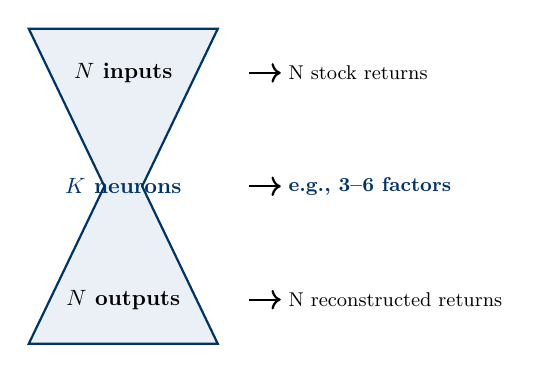
\begin{tikzpicture}[scale=0.8, every node/.style={scale=0.8}]
  % Hourglass shape
  \fill[accentblue!10] (0,0) -- (3,0) -- (1.8,2.5) -- (1.2,2.5) -- cycle;
  \fill[accentblue!10] (1.2,2.5) -- (1.8,2.5) -- (3,5) -- (0,5) -- cycle;
  \draw[thick, darkblue] (0,0) -- (3,0) -- (1.8,2.5) -- (3,5) -- (0,5) -- (1.2,2.5) -- cycle;
  
  \node[font=\bfseries] at (1.5, 4.3) {$N$ inputs};
  \node[font=\bfseries, darkblue] at (1.5, 2.5) {$K$ neurons};
  \node[font=\bfseries] at (1.5, 0.7) {$N$ outputs};
  
  % Right side explanation
  \node[right, align=left, font=\small] at (4.0, 4.3) {N stock returns};
  \node[right, align=left, font=\small\bfseries, darkblue] at (4.0, 2.5) {e.g., 3--6 factors};
  \node[right, align=left, font=\small] at (4.0, 0.7) {N reconstructed returns};
  
  \draw[->, thick] (3.5, 4.3) -- (4.0, 4.3);
  \draw[->, thick] (3.5, 2.5) -- (4.0, 2.5);
  \draw[->, thick] (3.5, 0.7) -- (4.0, 0.7);
\end{tikzpicture}
\end{center}

\vspace{0.3em}
\begin{itemize}
    \item The network \emph{cannot} simply memorize all $N$ returns through $K \ll N$ neurons
    \item It must learn a \textbf{compressed representation} that preserves the most important information
    \item The ``important information'' is precisely the \textbf{common factor structure}
    \item Idiosyncratic noise gets discarded (it can't squeeze through the bottleneck)
\end{itemize}
\end{frame}
%
%..................................................................
%
\begin{frame}{The Encoder--Decoder Paradigm}

\begin{columns}[T]
\column{0.48\textwidth}
\textbf{Encoder} ($N \to K$):
\[
h = g\!\left(b^{(0)} + W^{(0)} r_t\right)
\]
\begin{itemize}
    \item Takes $N$-dimensional return vector
    \item Compresses to $K$-dimensional hidden representation
    \item $W^{(0)} \in \R^{K \times N}$: encoder weights
    \item $g(\cdot)$: activation function
\end{itemize}

\column{0.48\textwidth}
\textbf{Decoder} ($K \to N$):
\[
\hat{r}_t = b^{(1)} + W^{(1)} h
\]
\begin{itemize}
    \item Takes $K$-dimensional hidden code
    \item Reconstructs $N$-dimensional return vector
    \item $W^{(1)} \in \R^{N \times K}$: decoder weights
    \item Output layer is \textbf{always linear} (no activation)
\end{itemize}
\end{columns}
\end{frame}
%
%..................................................................
%
\begin{frame}{The Encoder--Decoder Paradigm}
\textbf{Full model:}
\[
\hat{r}_t = b^{(1)} + W^{(1)}\, g\!\left(b^{(0)} + W^{(0)} r_t\right)
\]

\vspace{0.5cm}
\textbf{If $g$ is nonlinear} (ReLU): nonlinear autoencoder (more flexible than PCA).

\vspace{0.5cm}
\textbf{If $g$ is identity} ($g(x) = x$): linear autoencoder. \textbf{This is what we analyze now.}
\end{frame}
%__________________________________________________________________________
%
\subsection{Linear autoencoder = PCA}
%__________________________________________________________________________
%
\begin{frame}{The Linear Autoencoder}

Set the activation function to the identity: $g(x) = x$.

\begin{block}{Linear autoencoder with one hidden layer of $K$ neurons}
\vspace{0.5em}
\[
r_t = b^{(1)} + W^{(1)}\!\left(b^{(0)} + W^{(0)}\, r_t\right) + u_t
\]
\vspace{0.5em}
\end{block}

\vspace{0.3em}
\textbf{Parameters:}
\begin{center}
\renewcommand{\arraystretch}{1.2}
\begin{tabular}{lcl}
$W^{(0)}$ & $\in \R^{K \times N}$ & encoder weight matrix \\
$W^{(1)}$ & $\in \R^{N \times K}$ & decoder weight matrix \\
$b^{(0)}$ & $\in \R^{K \times 1}$ & encoder bias \\
$b^{(1)}$ & $\in \R^{N \times 1}$ & decoder bias \\
\end{tabular}
\end{center}

\vspace{0.3em}
\textbf{Total parameters:} $K(1+N) + N(1+K) = 2NK + N + K$

\end{frame}
%
%..................................................................
%
\begin{frame}{Expanding the Model}

Expand the parentheses:
\[
r_t = \underbrace{b^{(1)} + W^{(1)}b^{(0)}}_{\text{combined bias}} + \underbrace{W^{(1)}W^{(0)}}_{\text{rank-$K$ matrix}} r_t + u_t
\]

\vspace{0.5em}
\textbf{Observation:} The product $W^{(1)}W^{(0)}$ is an $N \times N$ matrix, but it has rank at most $K$ (because $W^{(1)}$ is $N \times K$ and $W^{(0)}$ is $K \times N$).

\vspace{0.5em}
\textbf{So the autoencoder projects $r_t$ onto a $K$-dimensional subspace, adds a bias, and tries to reconstruct $r_t$.}

\vspace{0.5em}
Compare with the factor model:
\[
r_t = \alpha + \underbrace{\beta}_{\text{$N \times K$}} \underbrace{f_t}_{\text{$K \times 1$}} + u_t
\]

The autoencoder learns both $\beta$ (through $W^{(1)}$) and $f_t$ (through $W^{(0)}r_t$) simultaneously!
\end{frame}
%
%..................................................................
%
\begin{frame}{The Optimization Problem}

\textbf{Training objective:} Minimize reconstruction error over all time periods.

\begin{block}{Optimization Equation}
\vspace{0.5em}
\[
\min_{b, W} \sum_{t=1}^{T} \left\| r_t - \left[ b^{(1)} + W^{(1)}\!\left(b^{(0)} + W^{(0)}\, r_t\right) \right] \right\|^2
\]
\vspace{0.5em}
\end{block}

In matrix notation (stacking over time):
\[
\min_{b, W} \left\| R - \left[ b^{(1)}\bm{1}' + W^{(1)}\!\left(b^{(0)}\bm{1}' + W^{(0)} R\right) \right] \right\|_F^2
\]

where $\|\cdot\|_F$ is the Frobenius norm, $\bm{1}$ is a $T \times 1$ vector of ones.

\vspace{0.5em}
\textbf{This is a least-squares problem.} For the linear case, we can solve it analytically by taking first-order conditions.
\end{frame}
%
%..................................................................
%
\begin{frame}{The Optimization Problem}

\begin{block}{Optimal Solution}
The optimal solution to the optimization problem is given by:
\begin{align}
\hat{W}^{(1)} &= \hat{P}\, A \tag{i}\\[4pt]
\hat{W}^{(0)} &= \left(\hat{W}^{(1)\prime}\hat{W}^{(1)}\right)^{-1}\hat{W}^{(1)\prime} \tag{ii}\\[4pt]
\hat{b}^{(1)} &= \bar{r} - \hat{W}^{(1)}\hat{b}^{(0)} - \hat{W}^{(1)}\hat{W}^{(0)}\bar{r} \tag{iii}\\[4pt]
\hat{b}^{(0)} &= a \quad (\text{arbitrary constant}) \tag{iv}
\end{align}
where $A$ is any $K \times K$ nonsingular matrix, $a$ is an arbitrary scalar, $\bar{r} = \frac{1}{T}\sum_t r_t$, and $\hat{P}$ are the left singular vectors from the SVD of $\bar{R}$ (i.e., the PCA loadings).
\end{block}

\vspace{0.3em}
\textbf{Bottom line:} The decoder weights $\hat{W}^{(1)}$ are the PCA loadings (up to rotation $A$).
\end{frame}
%
%..................................................................
%
\begin{frame}{Proof -- Step 1: Eliminate the Bias Terms}

\textbf{Take the FOC with respect to $b^{(1)}$:}
\[
\frac{\partial}{\partial b^{(1)}} \left\| R - b^{(1)}\bm{1}' - W^{(1)}(b^{(0)}\bm{1}' + W^{(0)}R) \right\|_F^2 = 0
\]

Setting the derivative to zero:
\[
\left[R - b^{(1)}\bm{1}' - W^{(1)}(b^{(0)}\bm{1}' + W^{(0)}R)\right]\bm{1} = 0
\]

Solving for $b^{(1)}$:
\[
\hat{b}^{(1)} = \frac{1}{T}\left(R\bm{1} - TW^{(1)}b^{(0)} - W^{(1)}W^{(0)}R\bm{1}\right) = \bar{r} - W^{(1)}b^{(0)} - W^{(1)}W^{(0)}\bar{r}
\]

\textbf{Substituting back:}
\[
\min_{W} \left\| \underbrace{R - \bar{r}\bm{1}'}_{\bar{R}} - W^{(1)}W^{(0)}\underbrace{(R - \bar{r}\bm{1}')}_{\bar{R}} \right\|_F^2 = \min_{W} \left\| \bar{R} - W^{(1)}W^{(0)}\bar{R} \right\|_F^2
\]

The bias terms drop out! The problem reduces to demeaned returns $\bar{R}$.
\end{frame}
%
%..................................................................
%
\begin{frame}{Proof -- Step 1: Key Insight}

\begin{exampleblock}{What just happened?}
The bias terms $b^{(0)}$ and $b^{(1)}$ absorb the \textbf{mean return}. The remaining optimization involves only \textbf{demeaned} returns $\bar{R}$.
\end{exampleblock}

\vspace{0.5em}
This is exactly analogous to standard PCA, which is applied to the demeaned (or centered) data!

\vspace{0.5em}
\textbf{Note:} $b^{(0)}$ is arbitrary -- it can take any value $a$, and $b^{(1)}$ adjusts to compensate. Only the product matters:
\[
b^{(1)} + W^{(1)}b^{(0)} = \bar{r} - W^{(1)}W^{(0)}\bar{r} = (I - W^{(1)}W^{(0)})\bar{r}
\]

This is the part of the mean return that the rank-$K$ projection cannot explain.
\end{frame}
%
%..................................................................
%
\begin{frame}{Proof -- Step 2: Solve for $W^{(0)}$ Given $W^{(1)}$}

\textbf{Now minimize over $W^{(0)}$ with $W^{(1)}$ fixed:}
\[
\frac{\partial}{\partial W^{(0)}} \left\| \bar{R} - W^{(1)}W^{(0)}\bar{R} \right\|_F^2 = 0
\]

This gives:
\[
W^{(1)\prime}W^{(1)}W^{(0)}\bar{R}\bar{R}' - W^{(1)\prime}\bar{R}\bar{R}' = 0
\]

Assuming $W^{(1)\prime}W^{(1)}$ and $\bar{R}\bar{R}'$ have full rank, solve:
\[
\boxed{\hat{W}^{(0)} = \left(W^{(1)\prime}W^{(1)}\right)^{-1}W^{(1)\prime}}
\]

\vspace{0.5em}
\textbf{This is the Moore--Penrose pseudoinverse of $W^{(1)}$!}

The encoder is the ``optimal inverse'' of the decoder.
\end{frame}
%
%..................................................................
%
\begin{frame}{Proof -- Step 2: The Projection Matrix}

\textbf{Substituting $\hat{W}^{(0)}$ back:}
\[
W^{(1)}\hat{W}^{(0)} = W^{(1)}\left(W^{(1)\prime}W^{(1)}\right)^{-1}W^{(1)\prime} =: P_{W^{(1)}}
\]

$P_{W^{(1)}}$ is the \textbf{orthogonal projection matrix} onto the column space of $W^{(1)}$.

\vspace{0.5em}
So the objective becomes:
\[
\min_{W^{(1)}} \left\| \bar{R} - P_{W^{(1)}}\bar{R} \right\|_F^2
\]

\vspace{0.5em}
\begin{alertblock}{Equivalent formulation}
\textbf{Find the $K$-dimensional subspace (column space of $W^{(1)}$) such that projecting $\bar{R}$ onto it minimizes the reconstruction error.}
\end{alertblock}

This is \emph{exactly} the PCA problem!
\end{frame}
%
%..................................................................
%
\begin{frame}{Proof -- Step 3: Apply Eckart--Young--Mirsky}
\small
\textbf{Theorem (Eckart--Young--Mirsky):} The best rank-$K$ approximation of a matrix $M$ in Frobenius norm is obtained by its truncated SVD:
\[
M^{(K)} = \sum_{j=1}^{K} \sigma_j\, p_j\, q_j'
\]

\vspace{0.3em}
\textbf{In our case:} $M = \bar{R}$, and the best rank-$K$ approximation is $\hat{P}\hat{\Lambda}\hat{Q}$.

\vspace{0.5em}
The projection that achieves this is:
\[
P_{W^{(1)}}\bar{R} = \hat{P}\hat{\Lambda}\hat{Q}
\]

This is satisfied if and only if $W^{(1)} = \hat{P}\,A$ for any invertible $K \times K$ matrix $A$.

\vspace{0.5em}
\begin{exampleblock}{Why the rotation $A$?}
\begin{itemize}
    \item $P_{\hat{P}A} = P_{\hat{P}}$ for any invertible $A$ (same column space)
    \item The projection depends only on the \emph{subspace}, not on the specific basis
    \item This is the rotation indeterminacy we saw in Part A
\end{itemize}
\end{exampleblock}
\end{frame}
%
%..................................................................
%
\begin{frame}{Proof -- Step 3: Putting It Together}

Therefore:
\begin{align*}
\hat{W}^{(1)} &= \hat{P}\,A \qquad &&\text{(decoder = PCA loadings $\times$ rotation)}\\[6pt]
\hat{W}^{(0)} &= (\hat{W}^{(1)\prime}\hat{W}^{(1)})^{-1}\hat{W}^{(1)\prime} = A^{-1}\hat{P}' \qquad &&\text{(encoder = rotated pseudoinverse)}\\[6pt]
\hat{W}^{(0)}\bar{R} &= A^{-1}\hat{P}'\bar{R} = A^{-1}\hat{\Lambda}\hat{Q} \qquad &&\text{(encoded output = rotated PCA factors)}
\end{align*}

\vspace{0.5em}
\textbf{Reconstruction:}
\[
\hat{W}^{(1)}\hat{W}^{(0)}\bar{R} = (\hat{P}\,A)(A^{-1}\hat{\Lambda}\hat{Q}) = \hat{P}\hat{\Lambda}\hat{Q}
\]

The rotation $A$ cancels out in the final reconstruction! \hfill $\square$

\vspace{0.5em}
\begin{block}{Conclusion}
The linear autoencoder and PCA produce \textbf{identical} reconstructions $\hat{r}_t$ and span the \textbf{same factor space}.
\end{block}
\end{frame}
%
%..................................................................
%
\begin{frame}{Summary of the Proof}

\begin{center}
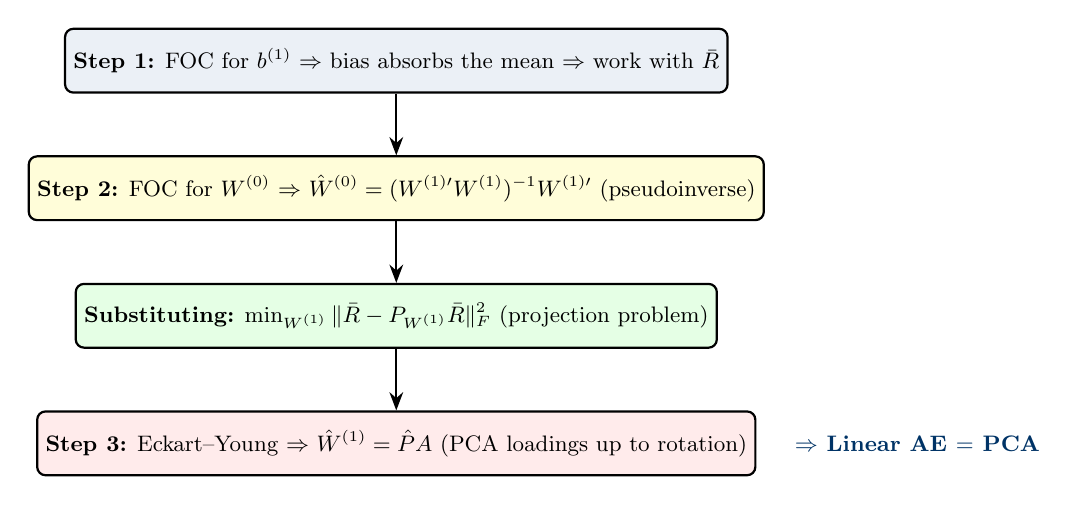
\begin{tikzpicture}[
    box/.style={draw, rounded corners=3pt, thick, minimum width=8cm, minimum height=0.9cm, align=center, font=\small},
    >=Stealth, scale=0.9, every node/.style={scale=0.9}
]
  \node[box, fill=accentblue!10] (s1) at (0, 0) {\textbf{Step 1:} FOC for $b^{(1)}$ $\Rightarrow$ bias absorbs the mean $\Rightarrow$ work with $\bar{R}$};
  
  \node[box, fill=yellow!15] (s2) at (0, -1.8) {\textbf{Step 2:} FOC for $W^{(0)}$ $\Rightarrow$ $\hat{W}^{(0)} = (W^{(1)\prime}W^{(1)})^{-1}W^{(1)\prime}$ (pseudoinverse)};
  
  \node[box, fill=green!10] (s3) at (0, -3.6) {\textbf{Substituting:} $\min_{W^{(1)}}\|\bar{R} - P_{W^{(1)}}\bar{R}\|_F^2$ (projection problem)};
  
  \node[box, fill=red!8] (s4) at (0, -5.4) {\textbf{Step 3:} Eckart--Young $\Rightarrow$ $\hat{W}^{(1)} = \hat{P}A$ (PCA loadings up to rotation)};
  
  \draw[->, thick] (s1) -- (s2);
  \draw[->, thick] (s2) -- (s3);
  \draw[->, thick] (s3) -- (s4);
  
  \node[right, font=\small\bfseries, darkblue] at (5.5, -5.4) {$\Rightarrow$ Linear AE $=$ PCA};
\end{tikzpicture}
\end{center}
\end{frame}
%__________________________________________________________________________
%
\subsection{From Autoencoder Back to Asset Pricing}
%__________________________________________________________________________
%
\begin{frame}{Where We Are and Where We're Going}

\textbf{What we proved (Proposition 1):} The optimal linear autoencoder satisfies
\[
\hat{W}^{(1)} = \hat{P} A, \qquad \hat{W}^{(0)} = \bigl(\hat{W}^{(1)\prime}\hat{W}^{(1)}\bigr)^{-1}\hat{W}^{(1)\prime}
\]

\vspace{0.5em}

\textbf{The question now:} We have been working with abstract matrices $W^{(0)}$, $W^{(1)}$, $\hat{P}$, $\hat{Q}$, $\hat{\Lambda}$\ldots

\vspace{0.5em}

\begin{alertblock}{The risk of losing sight of the economics}
At this point, it is easy to forget that we started from a very concrete \textbf{financial problem}: explaining stock returns through a small number of latent risk factors.
\end{alertblock}

\vspace{0.5em}

\textbf{Goal of these slides:} Carefully reconnect every autoencoder matrix to the original asset pricing quantities: \textbf{returns}, \textbf{factors}, and \textbf{factor loadings}.

\end{frame}
%
%..................................................................
%
\begin{frame}{Recall: The Factor Model We Want to Estimate}

The starting point is the \textbf{static linear factor model}:
\[
\boxed{r_t \;=\; \beta\, f_t \;+\; u_t}
\]

\vspace{0.3em}

\begin{center}
\renewcommand{\arraystretch}{1.4}
\begin{tabular}{c l l}
\hline
\textbf{Symbol} & \textbf{Dimension} & \textbf{Meaning} \\
\hline
$r_t$ & $N \times 1$ & Excess returns of $N$ stocks at time $t$ \\
$f_t$ & $K \times 1$ & Latent factor returns ($K \ll N$) \\
$\beta$ & $N \times K$ & Factor loadings (how each stock loads on each factor) \\
$u_t$ & $N \times 1$ & Idiosyncratic return (stock-specific noise) \\
\hline
\end{tabular}
\end{center}

\vspace{0.5em}

\textbf{The key economic content:}
\begin{itemize}
    \item $\beta$ tells us the \textbf{risk exposure} of each stock to each factor
    \item $f_t$ are the \textbf{common risk factors} driving all stocks together
    \item $u_t$ is diversifiable risk -- it washes out in large portfolios
\end{itemize}

\end{frame}
%
%..................................................................
%
\begin{frame}{Recall: The Linear Autoencoder We Trained}
\small
The one-layer linear autoencoder:
\[
\boxed{\hat{r}_t \;=\; b^{(1)} + W^{(1)}\!\bigl(b^{(0)} + W^{(0)} r_t\bigr)}
\]

\vspace{0.3em}

\begin{center}
\renewcommand{\arraystretch}{1.4}
\begin{tabular}{c l l}
\hline
\textbf{Symbol} & \textbf{Dimension} & \textbf{Role in the autoencoder} \\
\hline
$r_t$ & $N \times 1$ & Input (raw stock returns) \\
$W^{(0)}$ & $K \times N$ & Encoder weights (compress $N$ returns into $K$ codes) \\
$b^{(0)}$ & $K \times 1$ & Encoder bias \\
$h_t := b^{(0)} + W^{(0)} r_t$ & $K \times 1$ & Hidden code (compressed representation) \\
$W^{(1)}$ & $N \times K$ & Decoder weights (reconstruct $N$ returns from $K$ codes) \\
$b^{(1)}$ & $N \times 1$ & Decoder bias \\
$\hat{r}_t$ & $N \times 1$ & Output (reconstructed returns) \\
\hline
\end{tabular}
\end{center}

\vspace{0.3em}

\textbf{Now let's map each piece to the factor model.}

\end{frame}
%
%..................................................................
%
\begin{frame}{First: What Happens to the Bias Terms (Demeaning)}

Before identifying autoencoder matrices with factor model quantities, we need to understand a crucial simplification from Step 1 of the proof.

\vspace{0.3em}

The autoencoder reconstructs:
\[
\hat{r}_t = b^{(1)} + W^{(1)}\bigl(b^{(0)} + W^{(0)} r_t\bigr) = \underbrace{\bigl(b^{(1)} + W^{(1)}b^{(0)}\bigr)}_{\text{combined bias}} + \; W^{(1)}W^{(0)} r_t
\]

\vspace{0.3em}

Step 1 showed that the \textbf{optimal bias} satisfies:
\[
b^{(1)} + W^{(1)}b^{(0)} = \bar{r} - W^{(1)}W^{(0)}\bar{r} = (I - W^{(1)}W^{(0)})\,\bar{r}
\]

Substituting back:
\[
\hat{r}_t = (I - W^{(1)}W^{(0)})\bar{r} + W^{(1)}W^{(0)} r_t = \bar{r} + W^{(1)}W^{(0)}\underbrace{(r_t - \bar{r})}_{\bar{r}_t}
\]
\end{frame}
%
%..................................................................
%
\begin{frame}{First: What Happens to the Bias Terms (Demeaning)}

\begin{block}{The key consequence}
The bias absorbs the mean return $\bar{r}$. The weight matrices $W^{(1)}$ and $W^{(0)}$ only need to model the \textbf{demeaned returns} $\bar{r}_t = r_t - \bar{r}$. This is why we work on $\bar{R}$ (the matrix of demeaned returns), and exactly mirrors PCA, which also operates on centered data.
\end{block}

\end{frame}
%
%..................................................................
%
\begin{frame}{Why the Demeaning Matters Economically}

The decomposition from the previous slide is:
\[
\hat{r}_t = \underbrace{\bar{r}}_{\text{average return}} + \;\underbrace{W^{(1)}W^{(0)}\bar{r}_t}_{\text{time-varying part}}
\]

\vspace{0.3em}

This has a natural economic interpretation:

\vspace{0.3em}

\begin{center}
\renewcommand{\arraystretch}{1.5}
\begin{tabular}{c l}
\hline
\textbf{Term} & \textbf{Economic meaning} \\
\hline
$\bar{r}$ & Unconditional expected excess return of each stock \\
$\bar{r}_t = r_t - \bar{r}$ & Surprise: deviation of returns from their long-run average \\
$W^{(1)}W^{(0)}\bar{r}_t$ & The part of the surprise explained by $K$ common factors \\
\hline
\end{tabular}
\end{center}

\vspace{0.5em}

\textbf{From now on}, we focus on the demeaned returns $\bar{r}_t$ and study the product $W^{(1)}W^{(0)}$. This is where the factor structure lives.

%\vspace{0.3em}

%\begin{exampleblock}{Analogy}
%Think of $\bar{r}$ as the ``baseline temperature'' of each %stock. The factor model explains why temperatures %\textit{fluctuate} around the baseline -- that is, what common shocks drive stocks to move together on a given day.
%\end{exampleblock}

\end{frame}
%
%..................................................................
%
\begin{frame}{Why $\hat{W}^{(1)}$ Are the Factor Loadings: The Structural Argument}

Working with demeaned returns, the autoencoder reconstruction is:
\[
\hat{\bar{r}}_t \;=\; \hat{W}^{(1)} \;\cdot\; \hat{W}^{(0)} \bar{r}_t
\]

Now \textbf{define} $\hat{f}_t := \hat{W}^{(0)} \bar{r}_t$, which is a $K \times 1$ vector. Then we can write:
\[
\hat{\bar{r}}_t \;=\; \hat{W}^{(1)} \; \hat{f}_t
\]

Compare this side-by-side with the factor model:

\vspace{0.3em}

\begin{center}
\renewcommand{\arraystretch}{1.6}
\begin{tabular}{c @{\hskip 2em} c}
\textbf{Factor model} & \textbf{Autoencoder} \\
\hline
$r_t = \beta \, f_t + u_t$ & $\hat{\bar{r}}_t = \hat{W}^{(1)} \hat{f}_t$ \\
$\beta$ is $N \times K$ & $\hat{W}^{(1)}$ is $N \times K$ \\
$f_t$ is $K \times 1$ & $\hat{f}_t$ is $K \times 1$ \\
$\beta$ multiplies the factors & $\hat{W}^{(1)}$ multiplies the factors \\
\hline
\end{tabular}
\end{center}
\end{frame}
%
%..................................................................
%
\begin{frame}{Why $\hat{W}^{(1)}$ Are the Factor Loadings: The Structural Argument}

\begin{block}{The identification}
The two equations have \textbf{identical algebraic structure}. In both cases, an $N \times K$ matrix multiplies a $K \times 1$ vector to produce reconstructed returns. In the factor model that matrix is $\beta$; in the autoencoder it is $\hat{W}^{(1)}$. Therefore $\hat{W}^{(1)}$ \textit{is} the autoencoder's estimate of the factor loadings:
\vspace{-0.3em}
\[
\hat{W}^{(1)} \;\longleftrightarrow\; \hat{\beta}
\]
\end{block}
\small
To see this concretely, write the equation \textbf{for a single stock} $i$. The $i$-th row of $\hat{\bar{r}}_t = \hat{W}^{(1)}\hat{f}_t$ gives:
\[
\hat{\bar{r}}_{i,t} = \hat{W}^{(1)}_{i1}\,\hat{f}_{1,t} + \hat{W}^{(1)}_{i2}\,\hat{f}_{2,t} + \cdots + \hat{W}^{(1)}_{iK}\,\hat{f}_{K,t}
\]

The $i$-th row of the factor model $r_t = \beta f_t + u_t$ gives:
\[
r_{i,t} = \beta_{i1}\,f_{1,t} + \beta_{i2}\,f_{2,t} + \cdots + \beta_{iK}\,f_{K,t} + u_{i,t}
\]

\vspace{0.3em}

\textbf{Each coefficient $\hat{W}^{(1)}_{ik}$ plays the exact same role as $\beta_{ik}$:} it measures the sensitivity of stock $i$'s return to factor $k$.

\end{frame}
%
%..................................................................
%
\begin{frame}{The Encoder Output \texorpdfstring{$=$}{=} Estimated Factors}
\small
\begin{block}{From the proof (Step 2)}
\vspace{-0.5em}
\[
\hat{W}^{(0)} = \bigl(\hat{W}^{(1)\prime}\hat{W}^{(1)}\bigr)^{-1}\hat{W}^{(1)\prime} = A^{-1}\hat{P}'
\]
\end{block}

\vspace{0.3em}

The \textbf{hidden code} (encoder output) at time $t$, ignoring bias terms, is:
\[
h_t \;=\; \hat{W}^{(0)}\, \bar{r}_t \;\longleftrightarrow\; \hat{f}_t \qquad (K \times 1)
\]

\vspace{0.3em}

\textbf{What is this object?} Each component of $\hat{f}_t$ is a \textbf{weighted average} of all $N$ stock returns:
\[
\hat{f}_{k,t} \;=\; \sum_{i=1}^{N} \hat{W}^{(0)}_{ki}\; r_{i,t}
\]

\begin{exampleblock}{Key economic interpretation}
Each factor is a \textbf{portfolio}: a linear combination of individual stock returns. The encoder has \textit{learned} which portfolio weights best summarize the common variation in returns. These factors are \textbf{tradeable} -- an investor could, in principle, hold these portfolios.
\end{exampleblock}

\end{frame}
%
%..................................................................
%
\begin{frame}{The Reconstruction \texorpdfstring{$=$}{=} Factor Model Fit}

Putting the two pieces together on demeaned returns:
\[
\hat{\bar{r}}_t \;=\; \underbrace{\hat{W}^{(1)}}_{\hat{\beta}\;(N \times K)}\; \underbrace{\hat{W}^{(0)} \bar{r}_t}_{\hat{f}_t\;(K \times 1)} \;=\; \hat{\beta}\; \hat{f}_t
\]

\vspace{0.3em}

And adding back the mean (which the bias absorbed):
\[
\boxed{\hat{r}_t \;=\; \bar{r} \;+\; \sum_{k=1}^{K} \hat{\beta}_k\; \hat{f}_{k,t}}
\]

\vspace{0.3em}

\begin{center}
\textit{Each stock's return is approximated as its long-run average\\plus a linear combination of $K$ factor returns, weighted by that stock's loadings.}
\end{center}
\end{frame}
%
%..................................................................
%
\begin{frame}{The Reconstruction \texorpdfstring{$=$}{=} Factor Model Fit}

The \textbf{residual} is the idiosyncratic component:
\[
\hat{u}_t \;=\; r_t - \hat{r}_t \;=\; r_t - \hat{\beta}\,\hat{f}_t
\]

This is the part of the return \textbf{not explained} by the $K$ common factors -- the diversifiable, stock-specific risk (see Appendix).

\end{frame}
%
%..................................................................
%
\begin{frame}{The Complete Dictionary}

\begin{center}
\renewcommand{\arraystretch}{1.6}
\begin{tabular}{c c c c}
\hline
\textbf{Autoencoder} & \textbf{Dimension} & \textbf{Factor Model} & \textbf{PCA (SVD of $\bar{R}$)} \\
\hline
$r_t$ (input) & $N \times 1$ & $r_t$ (stock returns) & $r_t$ \\[3pt]
$\hat{W}^{(1)}$ (decoder) & $N \times K$ & $\hat{\beta}$ (loadings) & $\hat{P}\,A$ \\[3pt]
$\hat{W}^{(0)} \bar{r}_t$ (encoder output) & $K \times 1$ & $\hat{f}_t$ (factors) & $A^{-1}\hat{\Lambda}\hat{Q}_t$ \\[3pt]
$\hat{W}^{(1)}\hat{W}^{(0)}\bar{r}_t$ (output) & $N \times 1$ & $\hat{\beta}\hat{f}_t$ (fitted return) & $\hat{P}\hat{\Lambda}\hat{Q}_t$ \\[3pt]
$r_t - \hat{r}_t$ (residual) & $N \times 1$ & $\hat{u}_t$ (idiosyncratic) & $\hat{U}_t$ \\[3pt]
$K$ (bottleneck width) & scalar & \# of factors & \# of PCs retained \\
\hline
\end{tabular}
\end{center}
\end{frame}
%
%..................................................................
%
\begin{frame}{The Complete Dictionary}

\begin{block}{The unifying insight}
The autoencoder bottleneck, the number of PCA components retained, and the number of latent factors in the asset pricing model are \textbf{the same object} viewed from three different perspectives.
\end{block}

\end{frame}
%
%..................................................................
%
\begin{frame}{Visual Summary: Three Views of the Same Model}

\begin{center}
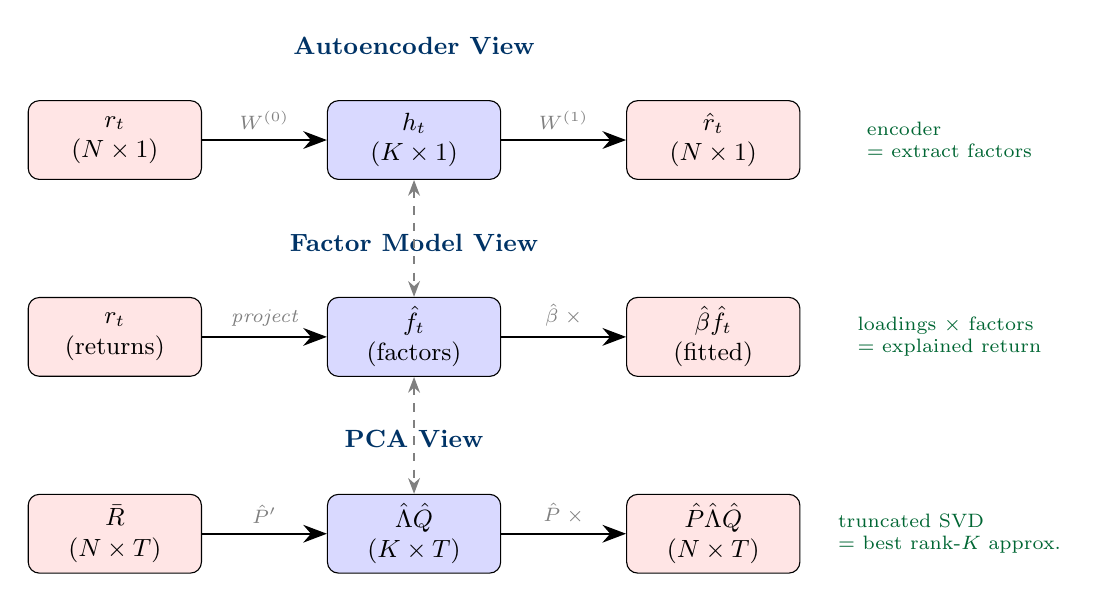
\begin{tikzpicture}[
    box/.style={draw, rounded corners=4pt, minimum width=2.2cm, minimum height=1cm, align=center, font=\small},
    arrow/.style={-{Stealth[length=3mm]}, thick},
    label/.style={font=\scriptsize\itshape, text=gray}
]

% --- Autoencoder view ---
\node[font=\bfseries\small, text=darkblue] at (0, 3.2) {Autoencoder View};
\node[box, fill=red!10] (ae_in) at (-3.8, 2) {$r_t$\\($N \times 1$)};
\node[box, fill=blue!15] (ae_hid) at (0, 2) {$h_t$\\($K \times 1$)};
\node[box, fill=red!10] (ae_out) at (3.8, 2) {$\hat{r}_t$\\($N \times 1$)};
\draw[arrow] (ae_in) -- node[above, label] {$W^{(0)}$} (ae_hid);
\draw[arrow] (ae_hid) -- node[above, label] {$W^{(1)}$} (ae_out);

% --- Factor model view ---
\node[font=\bfseries\small, text=darkblue] at (0, 0.7) {Factor Model View};
\node[box, fill=red!10] (fm_in) at (-3.8, -0.5) {$r_t$\\(returns)};
\node[box, fill=blue!15] (fm_fac) at (0, -0.5) {$\hat{f}_t$\\(factors)};
\node[box, fill=red!10] (fm_out) at (3.8, -0.5) {$\hat{\beta}\hat{f}_t$\\(fitted)};
\draw[arrow] (fm_in) -- node[above, label] {project} (fm_fac);
\draw[arrow] (fm_fac) -- node[above, label] {$\hat{\beta}\;\times$} (fm_out);

% --- PCA view ---
\node[font=\bfseries\small, text=darkblue] at (0, -1.8) {PCA View};
\node[box, fill=red!10] (pca_in) at (-3.8, -3) {$\bar{R}$\\($N \times T$)};
\node[box, fill=blue!15] (pca_mid) at (0, -3) {$\hat{\Lambda}\hat{Q}$\\($K \times T$)};
\node[box, fill=red!10] (pca_out) at (3.8, -3) {$\hat{P}\hat{\Lambda}\hat{Q}$\\($N \times T$)};
\draw[arrow] (pca_in) -- node[above, label] {$\hat{P}'$} (pca_mid);
\draw[arrow] (pca_mid) -- node[above, label] {$\hat{P}\;\times$} (pca_out);

% --- Equivalence arrows ---
\draw[{Stealth[length=2mm]}-{Stealth[length=2mm]}, dashed, gray, thick] (ae_hid.south) -- (fm_fac.north);
\draw[{Stealth[length=2mm]}-{Stealth[length=2mm]}, dashed, gray, thick] (fm_fac.south) -- (pca_mid.north);

% --- Labels on the right ---
\node[font=\scriptsize, text=darkgreen, align=left] at (6.8, 2) {encoder\\= extract factors};
\node[font=\scriptsize, text=darkgreen, align=left] at (6.8, -0.5) {loadings $\times$ factors\\= explained return};
\node[font=\scriptsize, text=darkgreen, align=left] at (6.8, -3) {truncated SVD\\= best rank-$K$ approx.};

\end{tikzpicture}
\end{center}

%\vspace{0.3em}

%All three are \textbf{mathematically identical} for the linear %case (Proposition 1).

\end{frame}
%__________________________________________________________________________
%
\subsection{Adding Non-Linearity}
%__________________________________________________________________________
%
\begin{frame}{What If We Add Nonlinearity?}

The linear autoencoder $=$ PCA. Now consider adding ReLU activation:

\vspace{0.5em}
\begin{columns}[T]
\column{0.48\textwidth}
\textbf{Linear autoencoder:}
\[
h_t = b^{(0)} + W^{(0)} r_t
\]
\[
\hat{r}_t = b^{(1)} + W^{(1)} h_t
\]
\begin{itemize}
    \item Equivalent to PCA
    \item Can only learn \textbf{linear} subspaces
    \item Global optimum (convex problem)
\end{itemize}

\column{0.48\textwidth}
\textbf{Nonlinear autoencoder:}
\[
h_t = \text{ReLU}\!\left(b^{(0)} + W^{(0)} r_t\right)
\]
\[
\hat{r}_t = b^{(1)} + W^{(1)} h_t
\]
\begin{itemize}
    \item \textbf{Generalizes} PCA
    \item Can learn \textbf{nonlinear manifolds}
    \item Multiple local optima (non-convex)
\end{itemize}
\end{columns}

\vspace{0.7em}
\textbf{What ReLU does:} $g(x) = \max(0, x)$ introduces \emph{piecewise linearity}. Different regions of the input space get different linear projections. This is far more flexible than a single global linear projection.
\end{frame}
%
%..................................................................
%
\begin{frame}{Nonlinear AE: Partitioning the Return Space}

\begin{center}
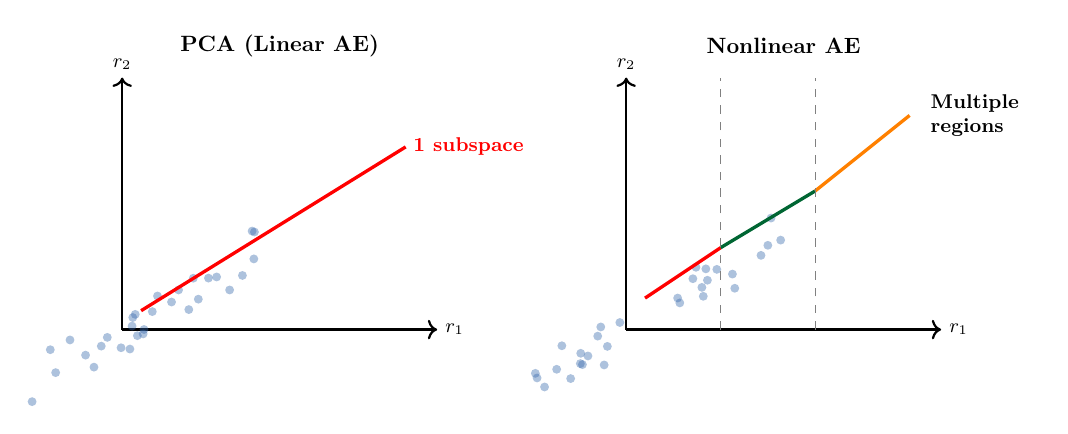
\begin{tikzpicture}[scale=0.8, every node/.style={scale=0.8}]
  % Left: PCA (single subspace)
  \node[font=\bfseries] at (2.5, 4.5) {PCA (Linear AE)};
  \draw[->, thick] (0,0) -- (5,0) node[right, font=\small] {$r_1$};
  \draw[->, thick] (0,0) -- (0,4) node[above, font=\small] {$r_2$};
  
  % Data cloud
  \foreach \i in {1,...,30}{
    \pgfmathsetmacro{\a}{0.5 + rand*2.0}
    \pgfmathsetmacro{\b}{\a*0.6 + rand*0.4}
    \fill[accentblue, opacity=0.4] (\a, \b) circle (2pt);
  }
  
  % Single linear subspace
  \draw[very thick, red] (0.3,0.3) -- (4.5, 2.9);
  \node[red, font=\small\bfseries, right] at (4.5, 2.9) {1 subspace};
  
  % Right: Nonlinear AE
  \node[font=\bfseries] at (10.5, 4.5) {Nonlinear AE};
  \draw[->, thick] (8,0) -- (13,0) node[right, font=\small] {$r_1$};
  \draw[->, thick] (8,0) -- (8,4) node[above, font=\small] {$r_2$};
  
  % Data cloud
  \foreach \i in {1,...,30}{
    \pgfmathsetmacro{\a}{0.5 + rand*2.0}
    \pgfmathsetmacro{\b}{\a*0.6 + rand*0.4}
    \fill[accentblue, opacity=0.4] ({\a+8}, \b) circle (2pt);
  }
  
  % Piecewise linear (ReLU regions)
  \draw[very thick, red] (8.3,0.5) -- (9.5, 1.3);
  \draw[very thick, darkgreen] (9.5, 1.3) -- (11.0, 2.2);
  \draw[very thick, orange] (11.0, 2.2) -- (12.5, 3.4);
  \node[font=\small\bfseries, right] at (12.5, 3.4) {\begin{tabular}{l}Multiple\\regions\end{tabular}};
  
  % ReLU regions
  \draw[dashed, gray] (9.5, 0) -- (9.5, 4);
  \draw[dashed, gray] (11.0, 0) -- (11.0, 4);
\end{tikzpicture}
\end{center}

\vspace{0.3em}
ReLU activation creates \textbf{different linear regimes} depending on which neurons are active ($> 0$) or inactive ($= 0$). Each regime has its own effective projection matrix.
\end{frame}
%
%..................................................................
%
\begin{frame}{Going Deeper: Multiple Hidden Layers}

The general recursive formula:
\[
r^{(l)} = g\!\left(b^{(l-1)} + W^{(l-1)} r^{(l-1)}\right), \qquad l = 1, \ldots, L
\]

\textbf{Adding depth} creates a \textbf{hierarchy of representations}:

\vspace{0.5em}
\begin{center}
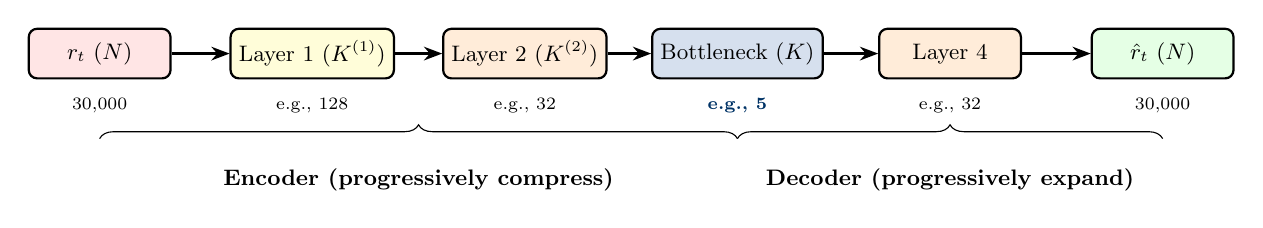
\begin{tikzpicture}[
    layer/.style={draw, rounded corners=3pt, thick, minimum width=2.0cm, minimum height=0.7cm, align=center, font=\small},
    >=Stealth, scale=0.9, every node/.style={scale=0.9}
]
  \node[layer, fill=red!10] (L0) at (0, 0) {$r_t$ ($N$)};
  \node[layer, fill=yellow!15] (L1) at (3, 0) {Layer 1 ($K^{(1)}$)};
  \node[layer, fill=orange!15] (L2) at (6, 0) {Layer 2 ($K^{(2)}$)};
  \node[layer, fill=accentblue!20] (BN) at (9, 0) {Bottleneck ($K$)};
  \node[layer, fill=orange!15] (L4) at (12, 0) {Layer 4};
  \node[layer, fill=green!10] (LO) at (15, 0) {$\hat{r}_t$ ($N$)};
  
  \draw[->, thick] (L0) -- (L1);
  \draw[->, thick] (L1) -- (L2);
  \draw[->, thick] (L2) -- (BN);
  \draw[->, thick] (BN) -- (L4);
  \draw[->, thick] (L4) -- (LO);
  
  % Size annotations
  \node[below, font=\scriptsize] at (0, -0.5) {30,000};
  \node[below, font=\scriptsize] at (3, -0.5) {e.g., 128};
  \node[below, font=\scriptsize] at (6, -0.5) {e.g., 32};
  \node[below, font=\scriptsize, darkblue] at (9, -0.5) {\textbf{e.g., 5}};
  \node[below, font=\scriptsize] at (12, -0.5) {e.g., 32};
  \node[below, font=\scriptsize] at (15, -0.5) {30,000};
  
  \draw[decorate, decoration={brace, amplitude=5pt}] (0, -1.2) -- (9, -1.2);
  \node[below, font=\small\bfseries] at (4.5, -1.5) {Encoder (progressively compress)};
  
  \draw[decorate, decoration={brace, amplitude=5pt}] (9, -1.2) -- (15, -1.2);
  \node[below, font=\small\bfseries] at (12, -1.5) {Decoder (progressively expand)};
\end{tikzpicture}
\end{center}

\vspace{0.5em}
\textbf{Deep autoencoders substantially outperform PCA and linear autoencoders for image recognition tasks}.
\end{frame}
%
%..................................................................
%
\begin{frame}{Deep AE: What Each Layer Learns}

\textbf{Intuition from computer vision (transferable to finance):}

\vspace{0.5em}
\begin{center}
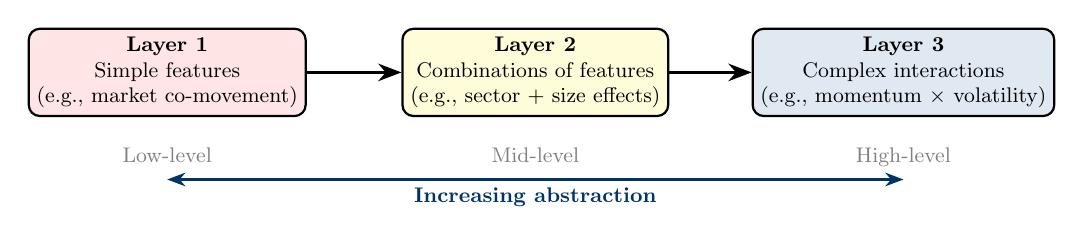
\begin{tikzpicture}[
    box/.style={draw, rounded corners, thick, minimum width=3.5cm, minimum height=1.2cm, align=center, font=\small},
    >=Stealth, scale=0.85, every node/.style={scale=0.85}
]
  \node[box, fill=red!10] (L1) at (0, 0) {\textbf{Layer 1}\\Simple features\\(e.g., market co-movement)};
  \node[box, fill=yellow!15] (L2) at (5.5, 0) {\textbf{Layer 2}\\Combinations of features\\(e.g., sector + size effects)};
  \node[box, fill=accentblue!15] (L3) at (11, 0) {\textbf{Layer 3}\\Complex interactions\\(e.g., momentum $\times$ volatility)};
  
  \draw[->, very thick] (L1) -- (L2);
  \draw[->, very thick] (L2) -- (L3);
  
  \node[below, font=\small, gray] at (0, -1.0) {Low-level};
  \node[below, font=\small, gray] at (5.5, -1.0) {Mid-level};
  \node[below, font=\small, gray] at (11, -1.0) {High-level};
  
  \draw[<->, thick, darkblue] (0, -1.6) -- node[below, font=\small\bfseries] {Increasing abstraction} (11, -1.6);
\end{tikzpicture}
\end{center}

\vspace{0.5em}
Each layer builds on the previous one to construct progressively more abstract and useful representations.

\vspace{0.3em}
\textbf{For asset pricing:}
\begin{itemize}
    \item Early layers: detect basic co-movement patterns
    \item Later layers: capture complex nonlinear interactions among characteristics
    \item Bottleneck: compressed factor representation
\end{itemize}
\end{frame}
%
%..................................................................
%
\begin{frame}{Number of Parameters per Architecture}

\textbf{Capacity} of the model grows with depth and width:

\vspace{0.5em}
\begin{center}
\renewcommand{\arraystretch}{1.3}
\begin{tabular}{llp{5.5cm}}
\toprule
\textbf{Model} & \textbf{Architecture (beta network)} & \textbf{Key feature} \\
\midrule
Linear AE & No hidden layer & Equivalent to PCA \\
CA0 & Single linear layer & Similar to IPCA \\
CA1 & 1 hidden layer (32 neurons) & Nonlinear, moderate capacity \\
CA2 & 2 hidden layers (32, 16) & Higher capacity, interactions \\
CA3 & 3 hidden layers (32, 16, 8) & Highest capacity \\
\bottomrule
\end{tabular}
\end{center}

\vspace{0.5em}
\textbf{Trade-off:} More parameters $\Rightarrow$ more flexibility $\Rightarrow$ but also more risk of overfitting.

\vspace{0.3em}
This is why \textbf{regularization} (L1 penalty, early stopping, ensemble) is critical -- as discussed in Lecture 1 and central to the paper's methodology.
\end{frame}
%
%..................................................................
%
\begin{frame}{A Note on the Output Layer}

\textbf{Important design choice:} The output layer of the autoencoder (both standard and conditional) is always \textbf{linear} (no activation function).

\vspace{0.5em}
Final output (Eq.\ 4 of the paper):
\[
G(r, b, W) = b^{(L)} + W^{(L)} r^{(L)}
\]

\textbf{Why no activation on the output?}
\begin{itemize}
    \item Returns $r_t$ can be positive or negative, and have no bounded range
    \item ReLU would clip negative values to zero -- destroying half the information
    \item A linear output allows the reconstruction to match the full range of returns
    \item The nonlinearity is applied in the \textbf{hidden layers} (encoder side), not the output
\end{itemize}

\vspace{0.5em}
\textbf{This also preserves the economic interpretation:} the output is a linear combination of factor returns weighted by loadings -- exactly a factor model.
\end{frame}
%
%..................................................................
%
\begin{frame}{Part 2 -- Summary}

\begin{enumerate}
    \item An \textbf{autoencoder} is a neural network that reconstructs its input through a bottleneck. The bottleneck forces a compressed representation.
    
    \vspace{0.3em}
    \item With \textbf{linear} activation and one hidden layer, the autoencoder is \textbf{exactly equivalent to PCA} (Proposition 1): decoder $=$ loadings, encoder output $=$ factors.
    
    \vspace{0.3em}
    \item The proof relies on three steps: (i) bias absorbs the mean, (ii) encoder is the pseudoinverse of decoder, (iii) Eckart--Young theorem gives PCA loadings as optimal decoder.
    
    \vspace{0.3em}
    \item Adding \textbf{nonlinearity} (ReLU) and \textbf{depth} (multiple layers) generalizes PCA to capture nonlinear patterns in the data.
    
    \vspace{0.3em}
    \item This establishes PCA as a \textbf{special case} of the autoencoder framework, and provides a smooth path from linear to nonlinear dimensionality reduction.
\end{enumerate}

\vspace{0.5em}
\textbf{Next (Part C):} How do we incorporate conditioning information ($z_{i,t-1}$) to allow time-varying betas? $\Rightarrow$ IPCA and the motivation for nonlinear models.
\end{frame}
%__________________________________________________________________________
%
\section{Part 3\\From Static to Conditional Models}
%__________________________________________________________________________
%
\begin{frame}{The Problem: Static Betas Are Inadequate}

\textbf{Standard factor models assume constant loadings:}

\begin{block}{Static Factor Model}
\vspace{-0.5em}
\[
  r_{i,t} \;=\; \bbeta' \bff_t \;+\; u_{i,t} \qquad \text{with } \bbeta \text{ \textbf{constant} across time}
\]
\vspace{-1em}
\end{block}

\bigskip
\textbf{But the real world is non-stationary:}
\begin{itemize}
  \item A tech startup in 2001 has very different risk characteristics than in 2010
  \item A bank's market beta \textbf{spikes} during financial crises
  \item Small-cap stocks may become large-cap over time, changing factor exposures
  \item Industry composition, leverage, and growth prospects all shift risk profiles
\end{itemize}

\begin{alertblock}{Result}
Fama-French 6-factor model achieves total $R^2 = -6.1\%$ on individual stocks (Table~1).
Static betas with ${\sim}30{,}000$ stocks, re-estimated only yearly, are badly stale.
\end{alertblock}

\end{frame}
%
%..................................................................
%
\begin{frame}{The Problem with Static Betas — A Concrete Example}

Consider two firms at the \textbf{same point in time}:

\begin{center}
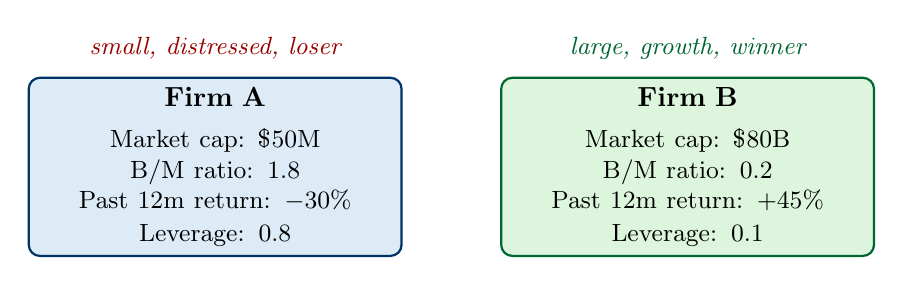
\begin{tikzpicture}
  \node[rectangle, rounded corners, draw=darkblue, thick, fill=lightblue,
        text width=4.5cm, align=center, minimum height=2.2cm] (A) at (0,0) {
    \textbf{Firm A} \\[4pt]
    \small Market cap: \$50M \\
    \small B/M ratio: 1.8 \\
    \small Past 12m return: $-30\%$ \\
    \small Leverage: 0.8
  };
  \node[rectangle, rounded corners, draw=darkgreen, thick, fill=lightgreen,
        text width=4.5cm, align=center, minimum height=2.2cm] (B) at (6,0) {
    \textbf{Firm B} \\[4pt]
    \small Market cap: \$80B \\
    \small B/M ratio: 0.2 \\
    \small Past 12m return: $+45\%$ \\
    \small Leverage: 0.1
  };
  \node[above=0.1cm of A, font=\small\itshape, text=darkred]
        {small, distressed, loser};
  \node[above=0.1cm of B, font=\small\itshape, text=darkgreen]
        {large, growth, winner};
\end{tikzpicture}
\end{center}

\bigskip
\textbf{Key question:} should Firm A and Firm B have the \emph{same} market beta? 
The \emph{same} sensitivity to a recession shock?

\medskip
\begin{alertblock}{The static model assumption}
In static factor models (FF, PCA), $\beta_i$ is \textbf{constant} for each firm.
Both firms get a single number estimated from 60 months of past returns.
This ignores all the information in their current observable attributes.
\end{alertblock}

\end{frame}
%
%..................................................................
%
\begin{frame}{Characteristics as Signals of Risk Exposure}

Economic theory and empirical evidence suggest that \textbf{observable firm attributes
predict how a firm responds to systematic shocks}:

\bigskip
\begin{center}
\begin{tabular}{p{3.2cm} p{4.5cm} p{4.5cm}}
\toprule
\textbf{Characteristic} & \textbf{Economic rationale} & \textbf{Expected effect on $\beta$} \\
\midrule
\textbf{Size} (market cap)
  & Small firms more exposed to liquidity and credit shocks
  & Small $\Rightarrow$ higher distress $\beta$ \\[6pt]
\textbf{Value} (B/M ratio)
  & High B/M firms have more assets in place, less flexibility
  & High B/M $\Rightarrow$ higher value $\beta$ \\[6pt]
\textbf{Momentum} (past returns)
  & Recent winners differ in investor attention, short-sale pressure
  & High mom $\Rightarrow$ different factor loading \\[6pt]
\textbf{Leverage}
  & More debt amplifies equity sensitivity to macro shocks
  & High lev $\Rightarrow$ higher market $\beta$ \\[6pt]
\textbf{Profitability}
  & Profitable firms less exposed to financial distress
  & High prof $\Rightarrow$ lower crash $\beta$ \\
\bottomrule
\end{tabular}
\end{center}
\end{frame}
%
%..................................................................
%
\begin{frame}{Characteristics as Signals of Risk Exposure}
\begin{block}{The key insight}
Characteristics are \textbf{proxies for latent risk exposures}. They contain information
about $\beta$ that is not captured by past returns alone.
\end{block}

\end{frame}
%
%..................................................................
%
\begin{frame}{Definition: Firm Characteristics}

\begin{block}{Definition}
A \textbf{firm characteristic} $z_{i,p,t-1}$ is any observable attribute of firm $i$,
measured at time $t-1$, that carries information about its future returns or risk
exposures.
\end{block}

\bigskip
Characteristics are collected into a vector for each firm and period:

$$z_{i,t-1} = \begin{pmatrix} z_{i,1,t-1} \\ z_{i,2,t-1} \\ \vdots \\ z_{i,P,t-1} \end{pmatrix} \in \mathbb{R}^P$$

\medskip
They come from \textbf{different data sources}, updated at different frequencies:

\begin{center}
\begin{tabular}{lcl}
\toprule
\textbf{Source} & \textbf{Frequency} & \textbf{Examples} \\
\midrule
Financial statements & Annual / Quarterly & B/M, leverage, profitability, investment \\
Market data         & Monthly            & Size, momentum, volatility, liquidity \\
\bottomrule
\end{tabular}
\end{center}

%\medskip
%In the paper (Gu, Kelly, Xiu 2020): $P = 94$ characteristics per firm per month.

\end{frame}
%
%..................................................................
%
\begin{frame}{Categories of Characteristics}

\begin{center}
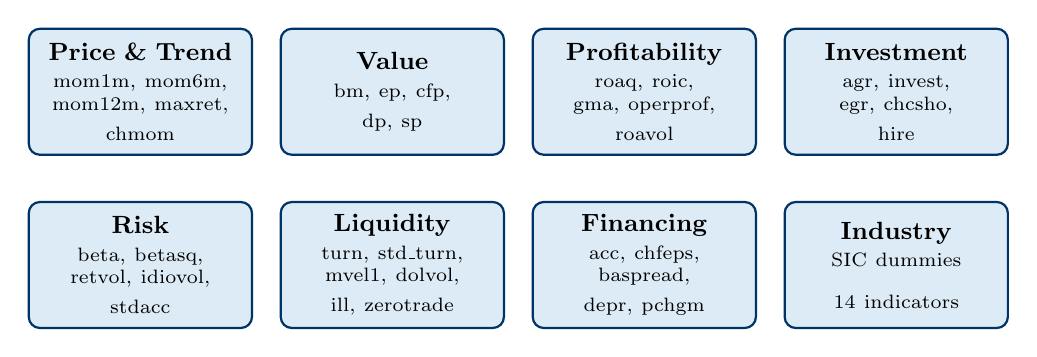
\begin{tikzpicture}[
  cat/.style={rectangle, rounded corners, draw=darkblue, thick,
              fill=lightblue, text width=2.6cm, align=center,
              minimum height=1.6cm, font=\small},
  item/.style={font=\scriptsize, align=left}
]

\node[cat] (pt) at (0, 2.2)   {\textbf{Price \& Trend}\\[2pt]\scriptsize mom1m, mom6m,\\ mom12m, maxret,\\ chmom};
\node[cat] (va) at (3.2, 2.2) {\textbf{Value}\\[2pt]\scriptsize bm, ep, cfp,\\ dp, sp};

\node[cat] (pr) at (6.4, 2.2) {\textbf{Profitability}\\[2pt]\scriptsize roaq, roic,\\ gma, operprof,\\ roavol};
\node[cat] (in) at (9.6, 2.2) {\textbf{Investment}\\[2pt]\scriptsize agr, invest,\\ egr, chcsho,\\ hire};

\node[cat] (ri) at (0, 0)     {\textbf{Risk}\\[2pt]\scriptsize beta, betasq,\\ retvol, idiovol,\\ stdacc};
\node[cat] (lq) at (3.2, 0)   {\textbf{Liquidity}\\[2pt]\scriptsize turn, std\_turn,\\ mvel1, dolvol,\\ ill, zerotrade};
\node[cat] (fi) at (6.4, 0)   {\textbf{Financing}\\[2pt]\scriptsize acc, chfeps,\\ baspread,\\ depr, pchgm};
\node[cat] (in2) at (9.6, 0)  {\textbf{Industry}\\[2pt]\scriptsize SIC dummies\\[4pt]\scriptsize 14 indicators};

%\node[above=0.05cm of pt, font=\tiny\itshape, text=darkred]  %{20 chars};
%\node[above=0.05cm of va, font=\tiny\itshape, text=darkred]  %{14 chars};
%\node[above=0.05cm of pr, font=\tiny\itshape, text=darkred]  %{13 chars};
%\node[above=0.05cm of in, font=\tiny\itshape, text=darkred]  %{10 chars};
%\node[below=0.05cm of ri,  font=\tiny\itshape, text=darkred] %{9 chars};
%\node[below=0.05cm of lq,  font=\tiny\itshape, text=darkred] %{7 chars};
%\node[below=0.05cm of fi,  font=\tiny\itshape, text=darkred] %{7 chars};
%\node[below=0.05cm of in2, font=\tiny\itshape, text=darkred] %{14 chars};
\end{tikzpicture}
\end{center}

\medskip
%\begin{exampleblock}{Update frequencies}
%61 annual \quad $|$ \quad 13 quarterly \quad $|$ \quad 20 monthly
%\end{exampleblock}

\end{frame}
%
%..................................................................
%
\begin{frame}{The Key Idea: Condition Betas on Characteristics}

\textbf{Let betas be a function of observable firm characteristics:}

\begin{block}{General Conditional Factor Model \normalfont(Equation 1 of the paper)}
\vspace{-0.5em}
\[
  r_{i,t} \;=\; \bbeta(\bz_{i,t-1})'\, \bff_t \;+\; u_{i,t}
\]
\vspace{-1em}
\end{block}

\medskip
\begin{tabular}{@{}ll@{}}
  $\bz_{i,t-1} \in \R^P$ & vector of $P$ lagged characteristics of firm $i$ \;(94 in the paper) \\[4pt]
  $\bbeta(\bz_{i,t-1}) \in \R^K$ & \textbf{conditional} factor loadings --- a function of characteristics \\[4pt]
  $\bff_t \in \R^K$ & latent factors (still to be estimated)
\end{tabular}
\end{frame}
%
%..................................................................
%
\begin{frame}{The Key Idea: Condition Betas on Characteristics}
\begin{exampleblock}{What this achieves}
As $\bz_{i,t-1}$ changes over time, betas \textbf{automatically update} every period.\\
No re-estimation needed --- just plug in new characteristics.\\
$P$ can be large (94 in the paper) --- many sources of conditioning information.
\end{exampleblock}

\medskip
\centerline{\color{navy}\textbf{Open question:} What is the functional form of $\bbeta(\cdot)$?}

\end{frame}
%
%..................................................................
%
\begin{frame}{First Solution: Linear Betas (IPCA)}

Kelly, Pruitt \& Su (2019) propose the simplest functional form: \textbf{linear}.

\begin{block}{Linear Beta Specification \normalfont(Equation 2 of the paper)}
\vspace{-0.5em}
\[
  \bbeta(\bz_{i,t-1})' \;=\; \bz_{i,t-1}'\, \Gamma
  \qquad \Gamma \in \R^{P \times K} \text{ constant}
\]
\vspace{-1em}
\end{block}

Each beta is a weighted combination of all 94 characteristics:
\[
  \beta_{i,k,t-1} \;=\; \gamma_k'\, \bz_{i,t-1} \;=\; \gamma_1 \cdot \text{size} + \gamma_2 \cdot \text{mom} + \gamma_3 \cdot \text{vol} + \cdots
\]

\medskip
\textbf{IPCA represents a major advance over static models:}

\smallskip
\centering
\begin{tabular}{l ccc}
  \toprule
  \textbf{Metric} ($K=6$, individual stocks) & \textbf{FF} & \textbf{PCA} & \textbf{IPCA} \\
  \midrule
  Total $R^2$ (\%)        & \textcolor{accent}{$-6.1$} & $3.9$ & \textcolor{dgreen}{\textbf{14.5}} \\
  Predictive $R^2$ (\%)   & \textcolor{accent}{$<0$}   & \textcolor{accent}{$<0$} & \textcolor{dgreen}{\textbf{0.30}} \\
  EW Sharpe Ratio          & \textcolor{accent}{$-0.21$}& $0.15$& \textcolor{dgreen}{\textbf{2.25}} \\
  \bottomrule
\end{tabular}

\end{frame}
%
%..................................................................
%
\begin{frame}{Why Characteristics $\Rightarrow$ Time-Varying Betas}

\begin{columns}[T]
\column{0.55\textwidth}

\textbf{Characteristics change over time for each firm:}
\begin{itemize}
  \item A small-cap stock grows $\to$ size changes $\to$ its $\beta$ updates
  \item Leverage increases $\to$ amplified exposure $\to$ $\beta$ adjusts
  \item Momentum reverses $\to$ new signal $\to$ new loadings
  \item The \textbf{same} mapping $\bbeta(\cdot)$ applies to all stocks at all times --- but each firm's $\bz$ changes
\end{itemize}

\begin{exampleblock}{Key insight}
Conditioning information captures both \textbf{cross-sectional} and \textbf{time-series} variation in risk exposures simultaneously.
\end{exampleblock}

\column{0.4\textwidth}
\centering
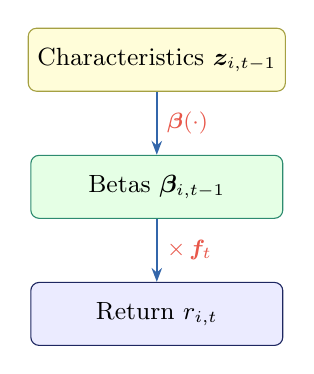
\begin{tikzpicture}[
  box/.style={draw, rounded corners=3pt, minimum width=3.2cm, minimum height=0.8cm, align=center, font=\small},
  arr/.style={-{Stealth[length=5pt]}, thick, accentblue}
]
  \node[box, fill=yellow!15, draw=yellow!60!black] (z) {Characteristics $\bz_{i,t-1}$};
  \node[box, fill=green!10, draw=dgreen, below=0.8cm of z] (beta) {Betas $\bbeta_{i,t-1}$};
  \node[box, fill=blue!8, draw=navy, below=0.8cm of beta] (r) {Return $r_{i,t}$};

  \draw[arr] (z) -- node[right, font=\footnotesize, text=accent] {$\bbeta(\cdot)$} (beta);
  \draw[arr] (beta) -- node[right, font=\footnotesize, text=accent] {$\times\, \bff_t$} (r);
\end{tikzpicture}

\bigskip
\centerline{\small\color{navy}\textbf{Open question:}}
\centerline{\small\color{navy}What is $\bbeta(\cdot)$?}
\end{columns}

\end{frame}
%
%..................................................................
%
\begin{frame}{But Is Linearity Enough?}

IPCA assumes $\bbeta(\bz) = \Gamma'\bz$ --- a linear map. \textbf{This rules out:}

\medskip
\begin{columns}[T]
\column{0.48\textwidth}
\begin{alertblock}{Interactions}
$\beta$ depends on $\text{size} \times \text{momentum}$\\
\footnotesize\textit{Linear treats each $z$ independently}
\end{alertblock}

\begin{alertblock}{Saturation}
$\beta$ flattens at extreme values of $z$\\
\footnotesize\textit{Linear extrapolates without bound}
\end{alertblock}

\column{0.48\textwidth}
\begin{alertblock}{Thresholds}
$\beta$ jumps at distress boundary\\
\footnotesize\textit{Linear is always smooth, monotonic}
\end{alertblock}

\begin{alertblock}{Curvature}
$\beta \propto z^2$ (beta-squared effect)\\
\footnotesize\textit{Linear: $\beta = \gamma z$ misses all curvature}
\end{alertblock}
\end{columns}

\begin{block}{Theoretical support for nonlinearity}
Leading asset pricing models --- Campbell--Cochrane (1999), Bansal--Yaron (2004), He--Krishnamurthy (2013), Santos--Veronesi (2004) --- all predict that the mapping from state variables to factor betas is \textbf{inherently nonlinear}. Linearity is a convenience, not a prediction of theory.
\end{block}

\end{frame}
%
%..................................................................
%
\begin{frame}{Next: The Conditional Autoencoder}

\textbf{Replace the linear mapping $\Gamma$ with a neural network:}

\bigskip
\centering
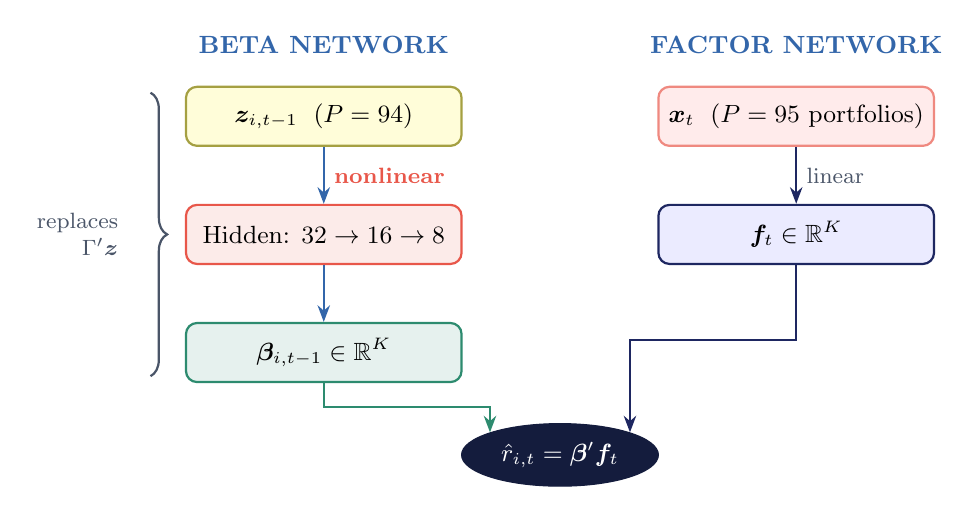
\begin{tikzpicture}[
  box/.style={draw, rounded corners=4pt, minimum width=3.5cm, minimum height=0.75cm, align=center, font=\small, thick},
  arr/.style={-{Stealth[length=6pt]}, thick},
  lbl/.style={font=\footnotesize, text=dgray}
]
  % ── Beta Network (left) ──
  \node[font=\small\bfseries, text=accentblue] at (-3,4.2) {BETA NETWORK};

  \node[box, fill=yellow!15, draw=yellow!60!black] (z) at (-3,3.3) {$\bz_{i,t-1}$ \;($P=94$)};
  \node[box, fill=accent!12, draw=accent] (hid) at (-3,1.8) {Hidden: $32 \to 16 \to 8$};
  \node[box, fill=dgreen!12, draw=dgreen, font=\small\bfseries] (beta) at (-3,0.3) {$\bbeta_{i,t-1} \in \R^K$};

  \draw[arr, accentblue] (z) -- node[right, lbl, text=accent] {\textbf{nonlinear}} (hid);
  \draw[arr, accentblue] (hid) -- (beta);

  % ── Factor Network (right) ──
  \node[font=\small\bfseries, text=accentblue] at (3,4.2) {FACTOR NETWORK};

  \node[box, fill=red!8, draw=accent!70] (x) at (3,3.3) {$\bm{x}_t$ \;($P=95$ portfolios)};
  \node[box, fill=blue!8, draw=navy, font=\small\bfseries] (f) at (3,1.8) {$\bff_t \in \R^K$};

  \draw[arr, navy] (x) -- node[right, lbl] {linear} (f);

  % ── Dot product ──
  \node[ellipse, draw=darknavy, fill=darknavy, text=white, minimum width=2.5cm, minimum height=0.7cm, font=\small\bfseries] (dot) at (0,-1) {$\hat{r}_{i,t} = \bbeta' \bff_t$};

  \draw[arr, dgreen] (beta.south) -- ++(0,-0.3) -| (dot.north west);
  \draw[arr, navy] (f.south) -- ++(0,-0.95) -| (dot.north east);

  % ── Brace annotation ──
  \draw[decorate, decoration={brace, amplitude=6pt, mirror}, thick, dgray]
    (-5.2, 0) -- (-5.2, 3.6) node[midway, left=8pt, font=\footnotesize, text=dgray, align=right] {replaces\\$\Gamma'\bz$};
\end{tikzpicture}

\end{frame}

% ============================================================
% SLIDE 10: SUMMARY
% ============================================================
\begin{frame}{Summary \& What's Next}

\begin{enumerate}
  \item \textbf{Static betas are inadequate:} return distributions are non-stationary; constant $\beta$ leads to $R^2 = -6.1\%$ for FF6.

  \item \textbf{Conditioning on characteristics} makes betas time-varying automatically: $\beta(\bz_{i,t-1})$ updates as firm attributes change.

  \item \textbf{IPCA} (linear $\beta = \Gamma'\bz$) is a huge improvement --- but both theory and data demand nonlinearity.

  \item \textbf{Deep conditional autoencoders} nearly double predictive $R^2$ and boost VW Sharpe ratios by 60\%.

  \item \textbf{Key result:} CA2 matches unrestricted ML prediction while imposing no-arbitrage $\Rightarrow$ characteristics proxy for \textbf{risk exposures}, not anomalies.
\end{enumerate}

\bigskip
\begin{block}{Next Lecture}
The Conditional Autoencoder: architecture in detail (CA0 $\to$ CA3), no-arbitrage restriction, end-to-end training via backpropagation, and full empirical results.
\end{block}

\end{frame}



%__________________________________________________________________________
%
\section{Appendix}
%__________________________________________________________________________
%
%__________________________________________________________________________
%
\subsection{Where Did $u_t$ Go?}
%__________________________________________________________________________
%
\begin{frame}{But Wait -- Where Did $u_t$ Go?}

A natural question arises from the side-by-side comparison:

\vspace{0.3em}

\begin{center}
\renewcommand{\arraystretch}{1.5}
\begin{tabular}{c @{\hskip 2em} c}
\textbf{Factor model} & \textbf{Autoencoder} \\
\hline
$r_t = \beta \, f_t + u_t$ & $\hat{\bar{r}}_t = \hat{W}^{(1)} \hat{f}_t$ \\
\hline
\end{tabular}
\end{center}

\vspace{0.3em}

\begin{alertblock}{The question}
The factor model has the idiosyncratic term $u_t$. The autoencoder does not. Where did it go?
\end{alertblock}

\vspace{0.3em}

\textbf{Answer:} The two equations describe \textit{different things}:
\begin{itemize}
    \item The factor model describes the \textbf{true data-generating process}: $r_t = \beta f_t + u_t$. The noise $u_t$ is always there in reality.
    \item The autoencoder produces a \textbf{reconstruction} $\hat{\bar{r}}_t$ -- its best attempt to approximate $\bar{r}_t$. It \textit{cannot} reproduce $u_t$ because the bottleneck of $K \ll N$ neurons does not have enough capacity to pass through $N$ independent noise terms.
\end{itemize}
\end{frame}
%
%..................................................................
%
\begin{frame}{But Wait -- Where Did $u_t$ Go?}

The term $u_t$ has not disappeared. It lives in the \textbf{reconstruction error}:
\[
\bar{r}_t \;=\; \underbrace{\hat{W}^{(1)}\hat{f}_t}_{\text{systematic part}} \;+\; \underbrace{\bigl(\bar{r}_t - \hat{W}^{(1)}\hat{f}_t\bigr)}_{\hat{u}_t \;\text{(residual)}}
\]

This equation now has \textit{exactly} the same form as $r_t = \beta f_t + u_t$.

\end{frame}
%
%..................................................................
%
\begin{frame}{The Bottleneck as a Filter for Noise}

\textbf{Why can't the autoencoder reproduce $u_t$?}

\vspace{0.3em}

The idiosyncratic errors $u_{1,t}, u_{2,t}, \ldots, u_{N,t}$ are (approximately) independent across stocks. To perfectly reproduce $N$ independent numbers, you would need $N$ degrees of freedom.

\vspace{0.3em}

But the bottleneck has only $K$ neurons (e.g., $K = 5$). So it can transmit at most $K$ independent pieces of information per time period.

\vspace{0.5em}

\begin{center}
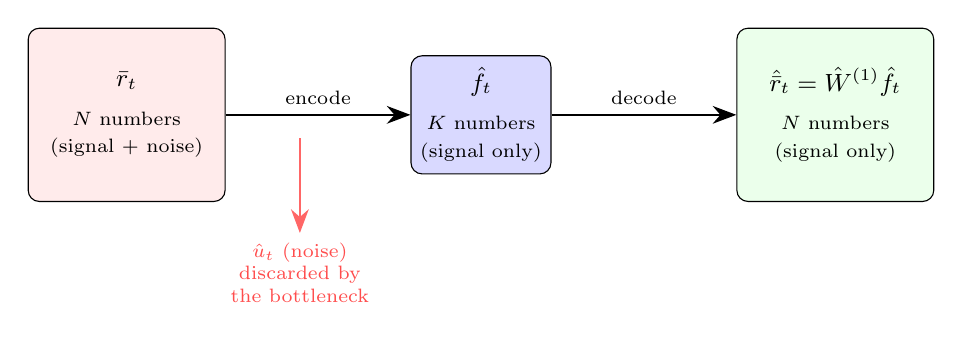
\begin{tikzpicture}[font=\small]
    % Left: signal + noise
    \node[draw, rounded corners, fill=red!8, minimum width=2.5cm, minimum height=2.2cm, align=center] (input) at (0,0) {$\bar{r}_t$\\[3pt]{\scriptsize $N$ numbers}\\[-1pt]{\scriptsize (signal $+$ noise)}};
    
    % Bottleneck
    \node[draw, rounded corners, fill=blue!15, minimum width=1.2cm, minimum height=1.5cm, align=center] (bottle) at (4.5,0) {$\hat{f}_t$\\[3pt]{\scriptsize $K$ numbers}\\[-1pt]{\scriptsize (signal only)}};
    
    % Right: reconstruction
    \node[draw, rounded corners, fill=green!8, minimum width=2.5cm, minimum height=2.2cm, align=center] (output) at (9,0) {$\hat{\bar{r}}_t = \hat{W}^{(1)}\hat{f}_t$\\[3pt]{\scriptsize $N$ numbers}\\[-1pt]{\scriptsize (signal only)}};
    
    \draw[-{Stealth[length=3mm]}, thick] (input) -- node[above]{\scriptsize encode} (bottle);
    \draw[-{Stealth[length=3mm]}, thick] (bottle) -- node[above]{\scriptsize decode} (output);
    
    % Noise arrow going down
    \draw[-{Stealth[length=3mm]}, thick, red!60] (2.2, -0.3) -- ++(0, -1.2) node[below, align=center, font=\scriptsize, text=red!70]{$\hat{u}_t$ (noise)\\discarded by\\the bottleneck};
\end{tikzpicture}
\end{center}
\end{frame}
%
%..................................................................
%
\begin{frame}{The Bottleneck as a Filter for Noise}

\begin{exampleblock}{This is a feature, not a bug}
The autoencoder's inability to reproduce noise is precisely what makes it useful. The bottleneck acts as a \textbf{filter}: it retains the common factor structure (signal) and discards the idiosyncratic variation (noise). This is the same principle behind PCA, and more broadly, behind all dimension reduction methods.
\end{exampleblock}

\end{frame}
%__________________________________________________________________________
%
\subsection{About the Rotation Indeterminacy}
%__________________________________________________________________________
%
\begin{frame}{The Rotation Indeterminacy: Why $A$ Doesn't Matter}

Proposition 1 says $\hat{W}^{(1)} = \hat{P}A$ for \textit{any} invertible $A$. Does this mean the solution is not unique?

\vspace{0.5em}

\textbf{Yes, but it doesn't matter.} Here is why.

\vspace{0.3em}

When we use $\hat{W}^{(1)} = \hat{P}A$, the encoder output becomes $\hat{W}^{(0)}\bar{r}_t = A^{-1}\hat{P}'\bar{r}_t$. So:
\[
\hat{r}_t = \underbrace{(\hat{P}A)}_{\text{loadings}} \underbrace{(A^{-1}\hat{P}'\bar{r}_t)}_{\text{factors}} = \hat{P}\,\hat{P}'\bar{r}_t
\]

The matrix $A$ \textbf{cancels out}. The reconstruction -- and therefore the model fit, the residuals, and any $R^2$ -- is identical regardless of $A$.
\end{frame}
%
%..................................................................
%
\begin{frame}{The Rotation Indeterminacy: Why $A$ Doesn't Matter}

\begin{exampleblock}{Physical analogy}
Think of choosing between Fahrenheit and Celsius. The \textit{temperature} is the same physical quantity; only the \textit{scale} changes. Similarly, $A$ changes the ``coordinate system'' within the factor space, but the \textbf{factor space itself} -- the set of risks that matter -- is uniquely determined.
\end{exampleblock}

\vspace{0.3em}

\textbf{What is uniquely identified:}
\begin{itemize}
    \item The $K$-dimensional factor \textbf{subspace} (column space of $\hat{\beta}$)
    \item The fitted returns $\hat{r}_t = \hat{\beta}\hat{f}_t$
    \item The residuals $\hat{u}_t = r_t - \hat{r}_t$
\end{itemize}

\end{frame}
%
%===================================================================================================
%
\end{document}
